\chapter{Descripción del Trabajo}
\label{cap:descripcionTrabajo}

Aquí comienza la descripción del trabajo realizado. Se deben incluir tantos capítulos como sea necesario para describir de la manera más completa posible el trabajo que se ha llevado a cabo. Como muestra la figura \ref{fig:sampleImage}, está todo por hacer.

\begin{figure}[H]
	\centering
	
\includegraphics[width = 0.5\textwidth]{Imagenes/Vectorial/Todo.pdf}
	\caption{Ejemplo de imagen}
	\label{fig:sampleImage}
\end{figure}

Si te sirve de utilidad, puedes incluir tablas para mostrar resultados, tal como se ve en la tabla \ref{tab:sampleTable}.


\begin{table}
	\centering
	\begin{tabular}{c|c|c}
		\textbf{Col 1} & \textbf{Col 2} & \textbf{Col 3} \\
		\hline\hline
		3 & 3.01 & 3.50\\
		6 & 2.12 & 4.40\\
		1 & 3.79 & 5.00\\
		2 & 4.88 & 5.30\\
		4 & 3.50 & 2.90\\
		5 & 7.40 & 4.70\\
		\hline
	\end{tabular}
	\caption{Tabla de ejemplo}
	\label{tab:sampleTable}
\end{table}
	
\section{Selección de librerías de OCR (Optical Character Recognition)}
Durante el desarrollo de este trabajo, se evaluaron varias herramientas de OCR para seleccionar la más adecuada para nuestras necesidades. Las herramientas probadas fueron OCRopus, EasyOCR y Tesseract. A continuación, se describe brevemente cada una de ellas.
\begin{enumerate}
	\item \textbf{OCRopus}
	\footnote{(repositorio github de OCRopus) \url{https://github.com/ocropus-archive/DUP-ocropy} }
	Es un sistema de OCR basado en redes neuronales con un enfoque modular.
	Principalmente esta disponible para Linux. Proporciona diferentes módulos para la binarización , segmentación ,generación del ground-truth y el entreno del modelo.
	Se ha utilizado la herramienta para reconocer la imagen de prueba pero el resultado fue que no consiguió reconocer ningún texto , por lo que fue descartado ya que las otras alternativas que hablaremos en adelante si que ha conseguido algo.
	Otras razones por la que esta herramienta fue descartado es que el lenguaje de programación principal con la que trabaja es \emph{python} y en nuestro proyecto trabajamos principalmente con \emph{c++}. Además la última actualización de esta librería fue en 16 de Diciembre de 2017
	
	\item \textbf{EasyOCR}
	EasyOCR es una biblioteca de reconocimiento óptico de caracteres (OCR) desarrollada en Python que facilita la extracción de texto de imágenes y documentos. Diseñada con el objetivo de ser fácil de usar y accesible, una de las características de EasyOCR es que es capaz de reconocer texto en más de 80 idiomas y soporta múltiples scripts, lo que la convierte en una herramienta versátil para diversas aplicaciones.
	La herramienta es fácil de usar y ofrece buenos resultados al reconocimiento.
	Proporciona gran variedad de modelos entrenados y también ofrece la opción de entrenar tu propio modelo.
	
	La herramienta en resumen se adapta muy bien a nuestras necesidades. El único problema esta en el idioma de programación con la que trabaja , al igual que OCRopus , EasyOCR está implementada con \emph{python} y nosotros con \emph{c++} , esto no supone un gran problema pero hemos encontrado una mejor solución.
	
	\item \textbf{Tesseract}
	
	Tesseract es una biblioteca de (OCR) de código abierto que se utiliza para convertir imágenes de texto en texto editable. Originalmente desarrollado por Hewlett-Packard en la década de 1980, Tesseract fue liberado como software de código abierto en 2005 y ha sido mantenido y mejorado por la comunidad, particularmente por Google, que ha contribuido significativamente a su desarrollo.
	
	Al igual que EasyOCR una de las características más destacadas de Tesseract es su capacidad para reconocer texto en múltiples idiomas y alfabetos, soportando más de 100 idiomas de forma nativa. Esto lo convierte en una herramienta versátil para aplicaciones globales que requieren la extracción de texto de documentos escritos en diferentes lenguas.
	
	Tesseract utiliza técnicas avanzadas de aprendizaje profundo y redes neuronales, lo que le permite alcanzar altos niveles de precisión en el reconocimiento de texto. Su arquitectura se basa en el uso de modelos de aprendizaje profundo entrenados con grandes conjuntos de datos, lo que mejora continuamente su rendimiento en diversas condiciones.
	
	El motor puede integrarse fácilmente en aplicaciones de procesamiento de imágenes y visión por computadora. Tesseract se utiliza comúnmente en combinación con bibliotecas como OpenCV para preprocesar imágenes antes de la etapa de reconocimiento, lo que mejora la precisión de los resultados.
	
	Además, Tesseract ofrece una API en varios lenguajes de programación, lo que facilita su integración en diferentes entornos de desarrollo y una de ellas es C++, por lo que esta herramienta cumple con todos los requisitos para nuestro proyecto y es la razón por la que hemos optado por Tesseract.
\end{enumerate}
\subsection{Pruebas y resultados de los OCR}
Para evaluar los resultados de los OCRs y hacer la elección del OCR a utilizar se tiene en cuenta el tiempo de ejecución necesario para reconocer los caractéres y el CER(Character Error Rate).


\textbf{CER (Character Error Rate)} \footnote{(Char Error Rate — PyTorch-Metrics 1.5.2 documentation)\url{https://lightning.ai/docs/torchmetrics/stable/text/char_error_rate.html} }
El CER es una métrica usada comúnmente para evaluar la precisión de un sistema de reconocimiento de caracteres (OCR) u otros sistemas que transcriba texto.El valor se obtiene calculando el número de errores a nivel de carácter dividido por el número total de caracteres en el texto de referencia.
Los errores pueden ser de:
\begin{enumerate}
	\item Sustituciones: Un carácter incorrecto reemplaza a uno correcto.
	\item Inserciones: Aparece un carácter extra que no debería estar.
	\item Eliminaciones: Falta un carácter que debería estar presente.
\end{enumerate}
La fórmula general para calcular el CER es:
	
	$CER = \frac{S+D+I}{N} $ 



Donde:

S es el número de sustituciones.

D es el número de eliminaciones.

I es el número de inserciones.

N es el número total de caracteres en el texto de referencia.





El CER se expresa como un valor entre 0 y 1 (o como porcentaje), donde 0 significa que no hubo errores (transcripción perfecta) , 1 (o 100) indica que todos los caracteres son incorrectos.


La prueba se ha hecho con 13 imágenes elegidas de forma que se considera más fácil de reconocer(a ojo humano)las imágenes con menor número de identificación.
Las imágenes se pueden encontrar en el repositorio del trabajo en OCRTests/images.
Se utiliza la libreria Jiwer\footnote{(Jiwer Usage)\url {https://jitsi.github.io/jiwer/usage/}} en python para los cálculos de CER, para más detalles se puede mirar el archivo Jiwer\_Cer.py situado en OCRTests.

En los resultados de los ocr se encontrará un valor llamado CER medio ,este valor se obtiene calculando el número total de errores a nivel de carácter encontrado en toda la batería de prueba divido entre el número total de caracteres de toda la batería de prueba.
\begin{enumerate}
	\item \textbf{Tesseract}
	
	
	Resultados del CER de cada imágen y el CER medio
	\begin{verbatim}
		{
			"1": 0.0,
			"2": 0.0625,
			"3": 0.5384615384615384,
			"4": 0.043478260869565216,
			"5": 0.2890625,
			"6": 0.025,
			"7": 0.75,
			"8": 0.9347826086956522,
			"9": 0.7209302325581395,
			"10": 1.0,
			"11": 0.05,
			"12": 0.35172413793103446,
			"13": 0.22988505747126436,
			"CER medio": 0.3842941796913226
		}
	\end{verbatim}
	El tiempo transcurrido para finalizar el OCR ha sido de 5539 milisegundos.
	\begin{figure}[H]
		\centering
		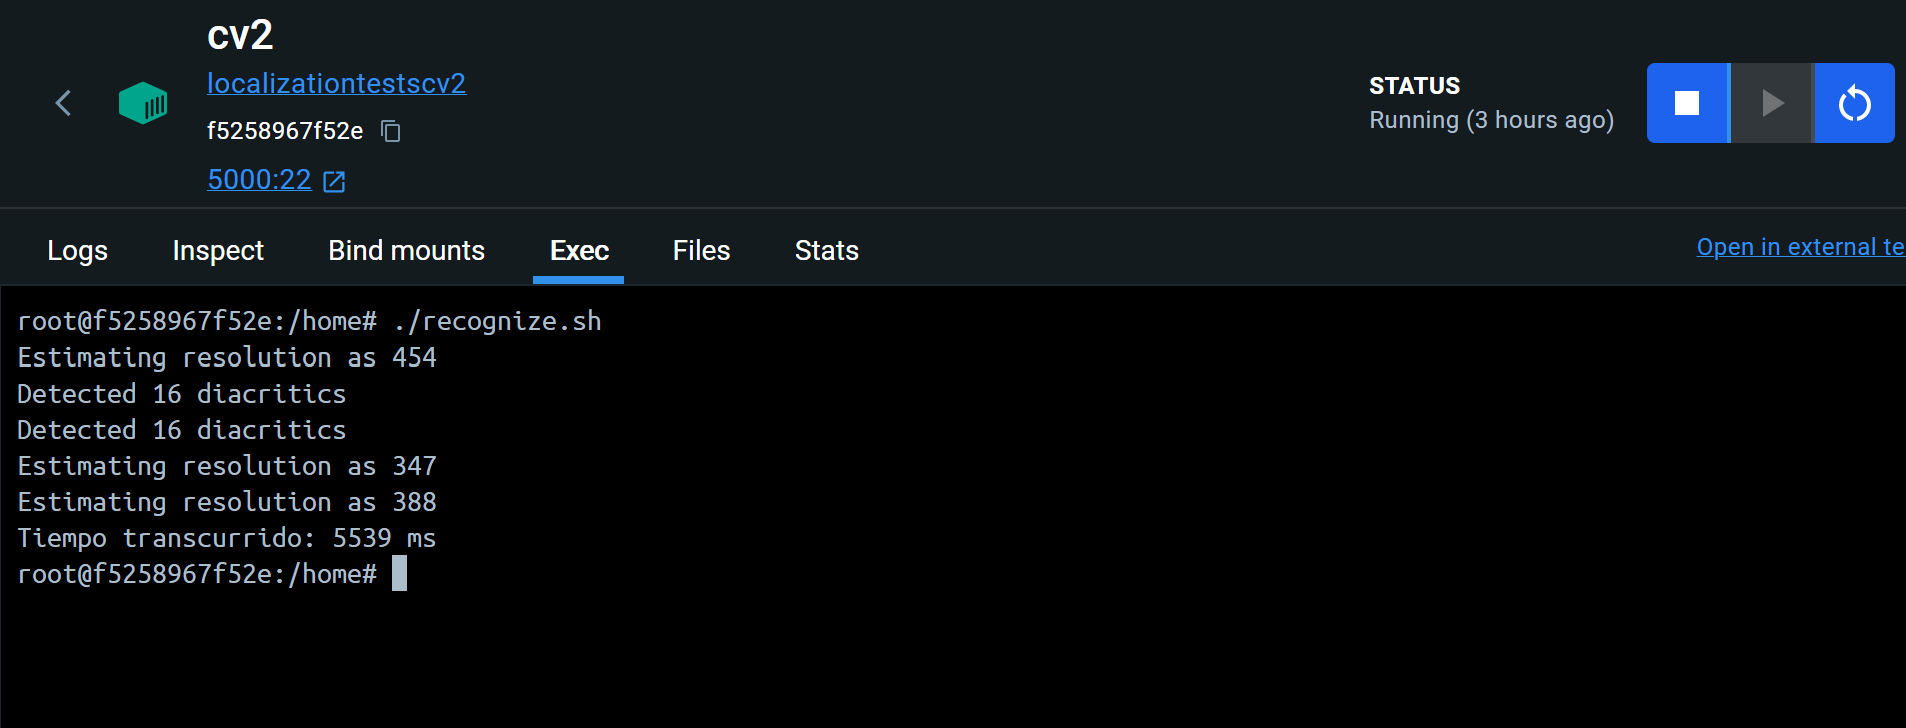
\includegraphics[width = 1\textwidth]{Imagenes/OCR/Tiempo_Tesseract.png}
		\caption{Tiempo transcurrido en la prueba usando Tesseract}
	\end{figure}
	\item \textbf{EasyOcr}
	
	Resultados del CER de cada imágen y el CER medio
	\begin{verbatim}
	
		{
			"1": 0.0,
			"2": 0.28125,
			"3": 0.21153846153846154,
			"4": 0.10869565217391304,
			"5": 0.0859375,
			"6": 0.025,
			"7": 0.0,
			"8": 0.6521739130434783,
			"9": 0.2558139534883721,
			"10": 0.8571428571428571,
			"11": 0.15,
			"12": 0.05517241379310345,
			"13": 0.3371647509578544,
			"CER medio": 0.23229919247215694
		}
	\end{verbatim}
	
		El tiempo transcurrido para finalizar el OCR ha sido de 204625 milisegundos.
	\begin{figure}[H]
		\centering
		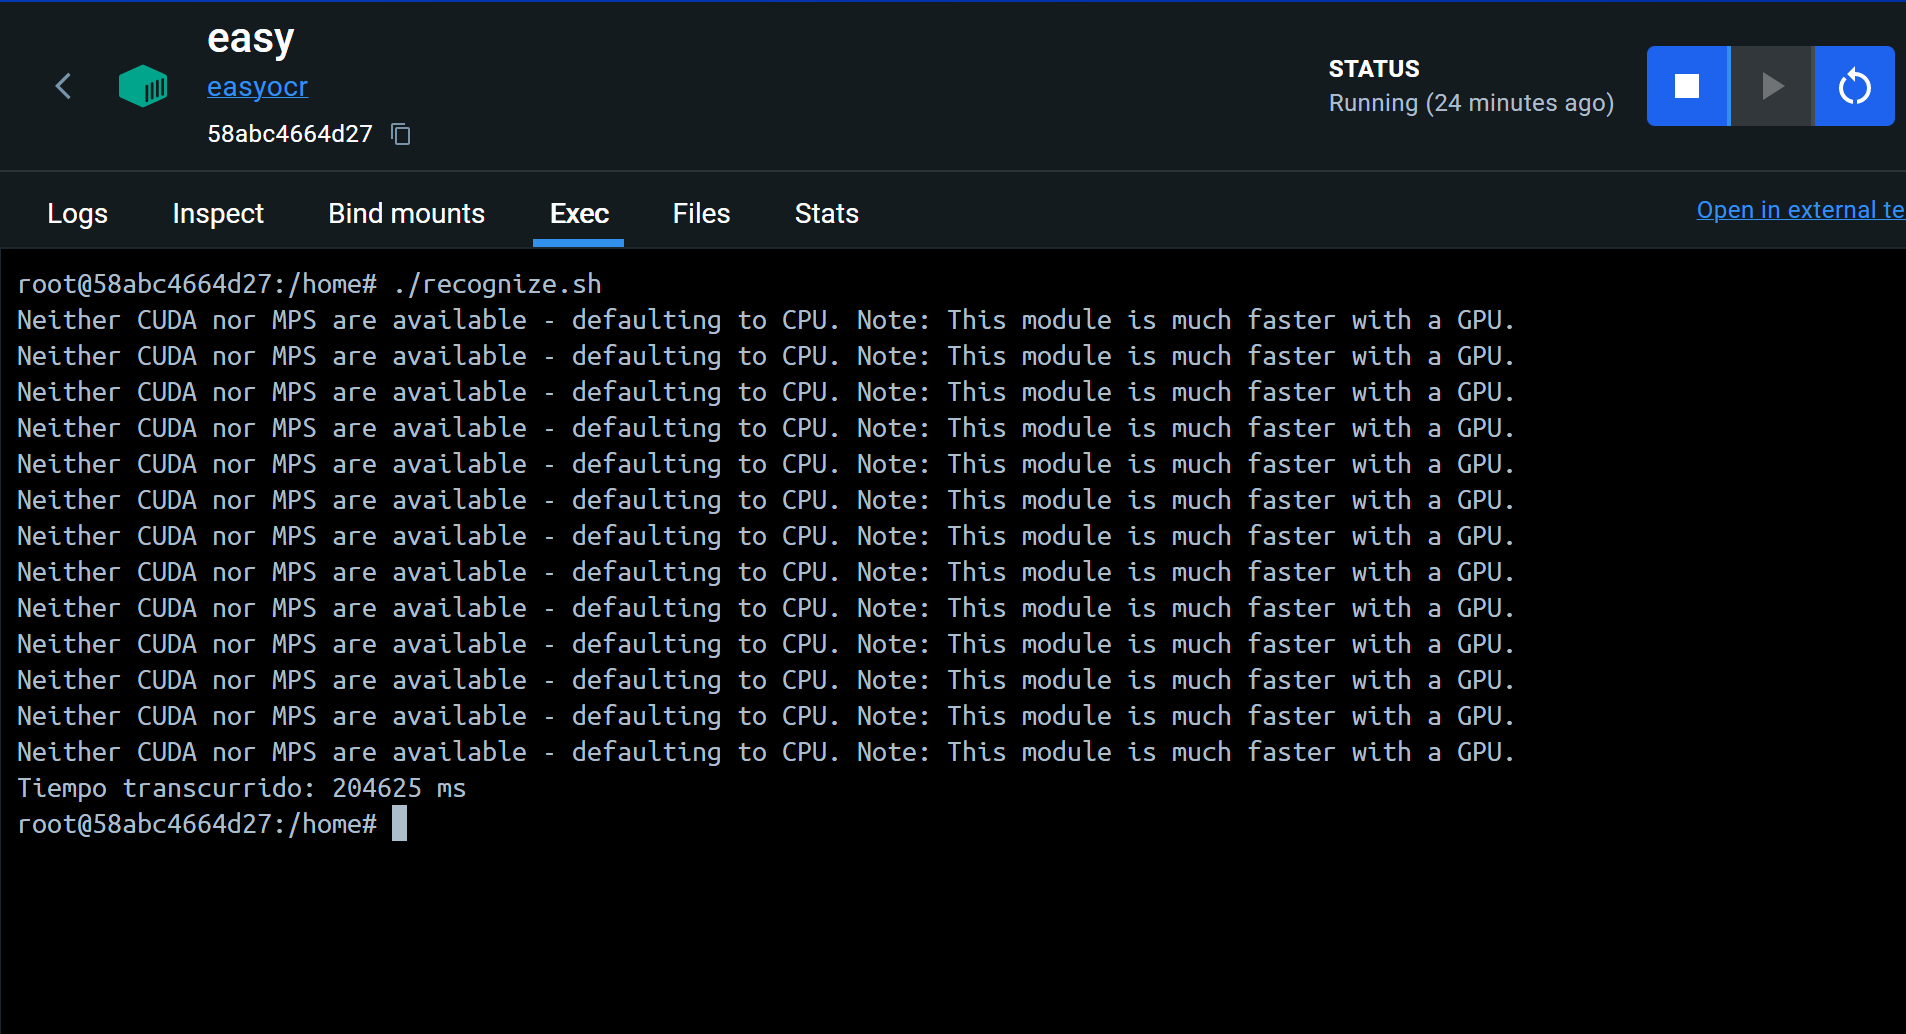
\includegraphics[width = 1\textwidth]{Imagenes/OCR/Tiempo_EasyOcr.png}
		\caption{Tiempo transcurrido en la prueba usando EasyOCR}
	\end{figure}
	
	\item \textbf{OCRopus}
	
		\begin{verbatim}
		
		{

		}
	\end{verbatim}
\end{enumerate}


Como se puede ver en los resultados obtenidos de los test realizados, tanto Tesseract y EasyOCR obtiene buenos resultados. Aunque EasyOCR obtiene un mejor CER medio en los resultados (0.23) que Tesseract (0.38), Tesseract es muchísimo más rápido que EasyOCR teniendo un 199086 milisegundo de adelanto que equivale a 3 minutos y medio. Por tanto decidimos seguir en adelante con Tesseract.



\section{Mejoras en el reconocimiento de texto en imágenes}
En este trabajo es muy importante que la entrada de los test sea correctos ya que todos nuestros test se basan en ello, por lo que se propone mejoras para aumentar la precisión del texto obtenido por el OCR disminuyendo el CER.

\textbf{Clasificación de imágenes de pruebas}

Para obtener más información sobre aquellos factores o características de las imágenes que puedan afectar al rendimiento y efectividad de la herramienta de OCR, se ha clasificado las imágenes en 5 categorías diferentes,la clasificación se ha hecho a ojo humano de forma subjetiva.
\begin{enumerate}
	\item Fondos simples.
		\begin{figure}[H]
		\centering
		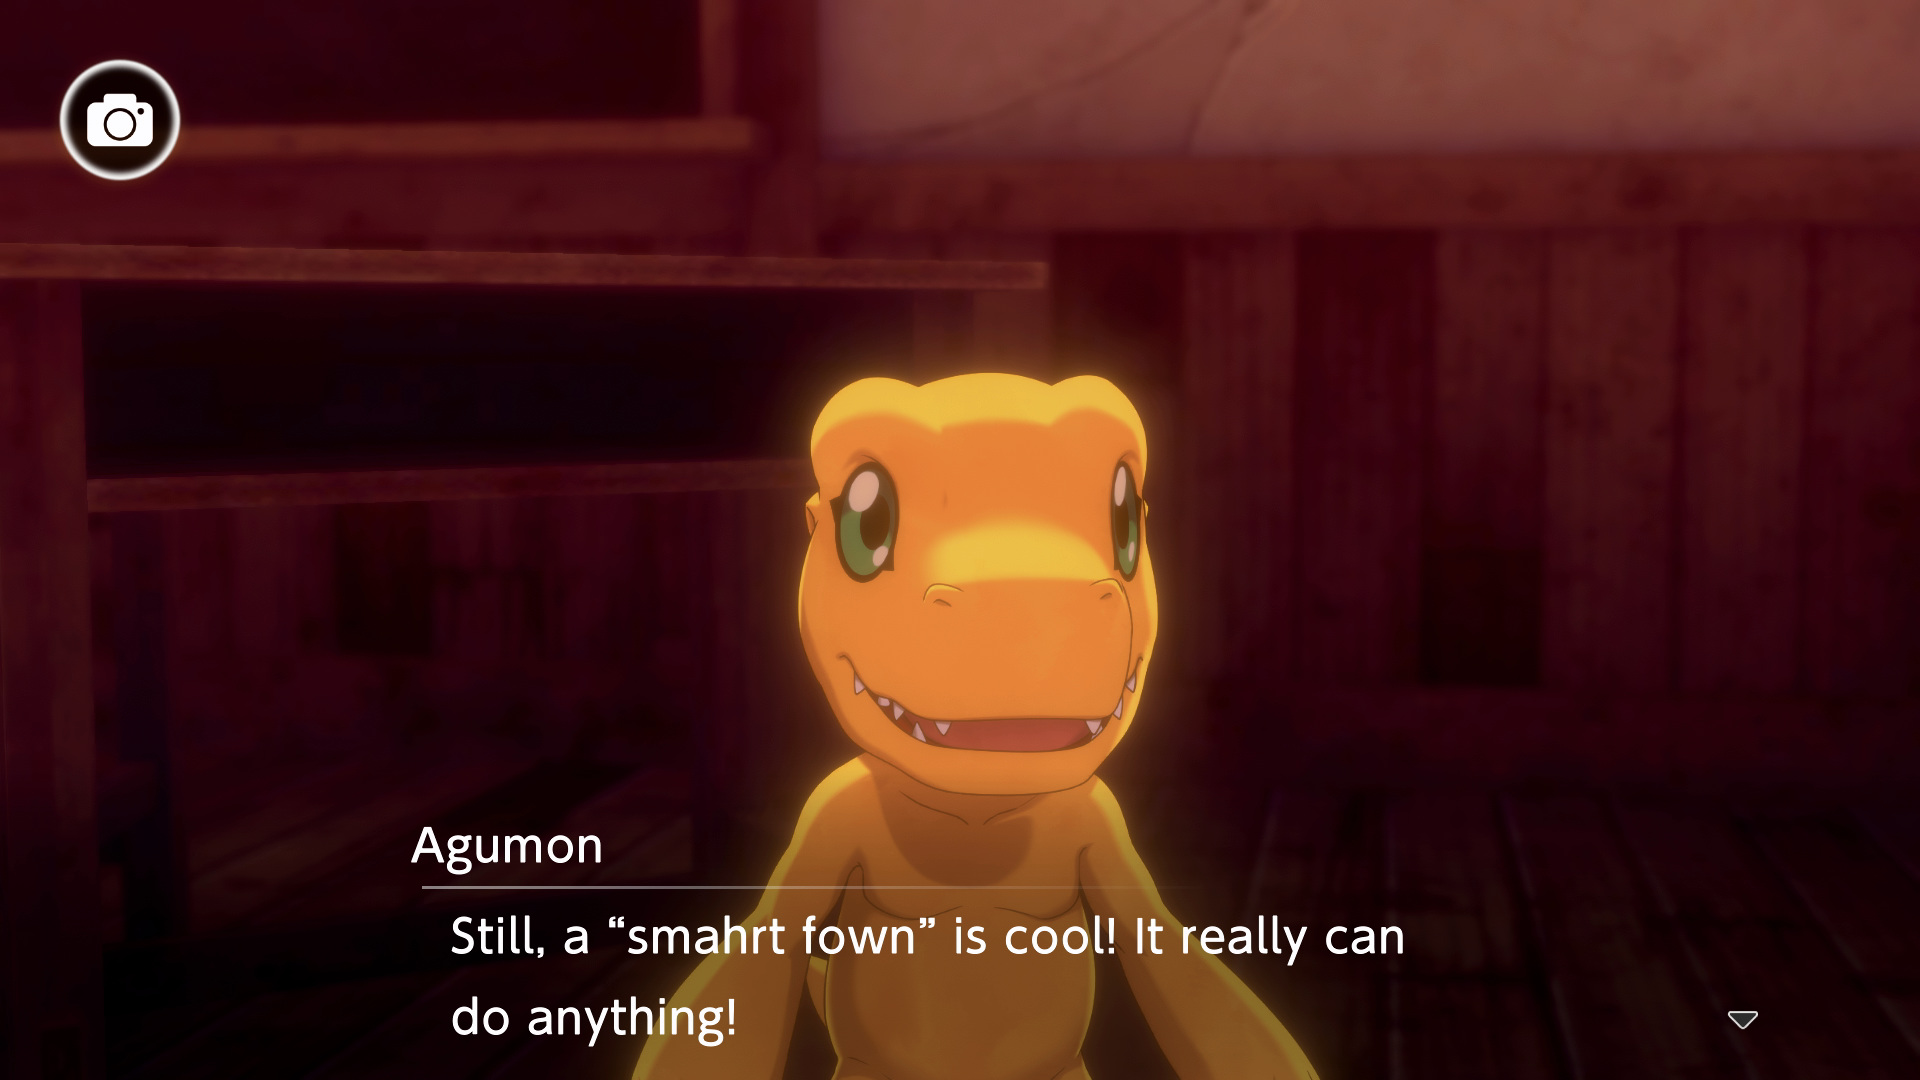
\includegraphics[width = 0.5\textwidth]{Imagenes/OCR/Simple.png}
		\caption{Ejemplo imagen fondos simples }
	\end{figure}
	
	\item Fondos complejos.
		\begin{figure}[H]
		\centering
		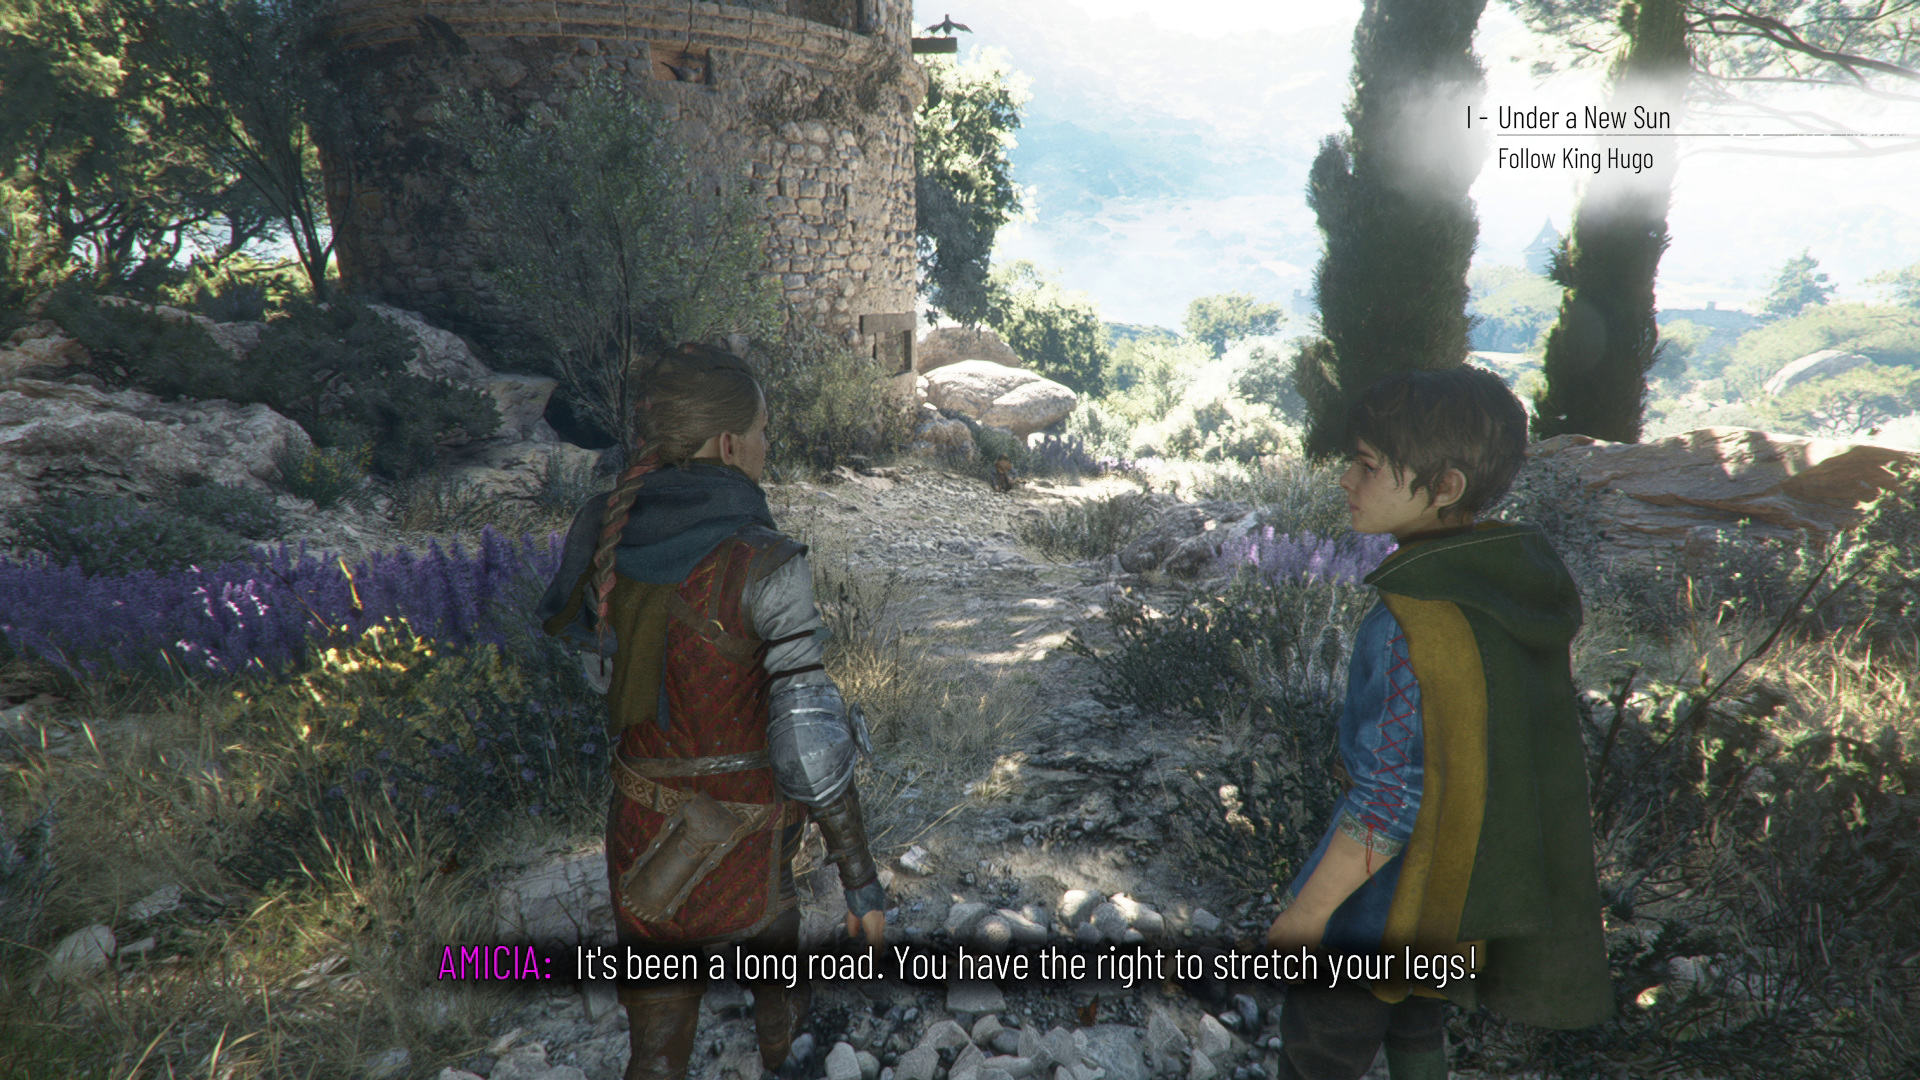
\includegraphics[width = 0.5\textwidth]{Imagenes/OCR/Complejo.png}
		\caption{Ejemplo imagen fondos complejos }
	\end{figure}
	\item PixelArt.
		\begin{figure}[H]
		\centering
		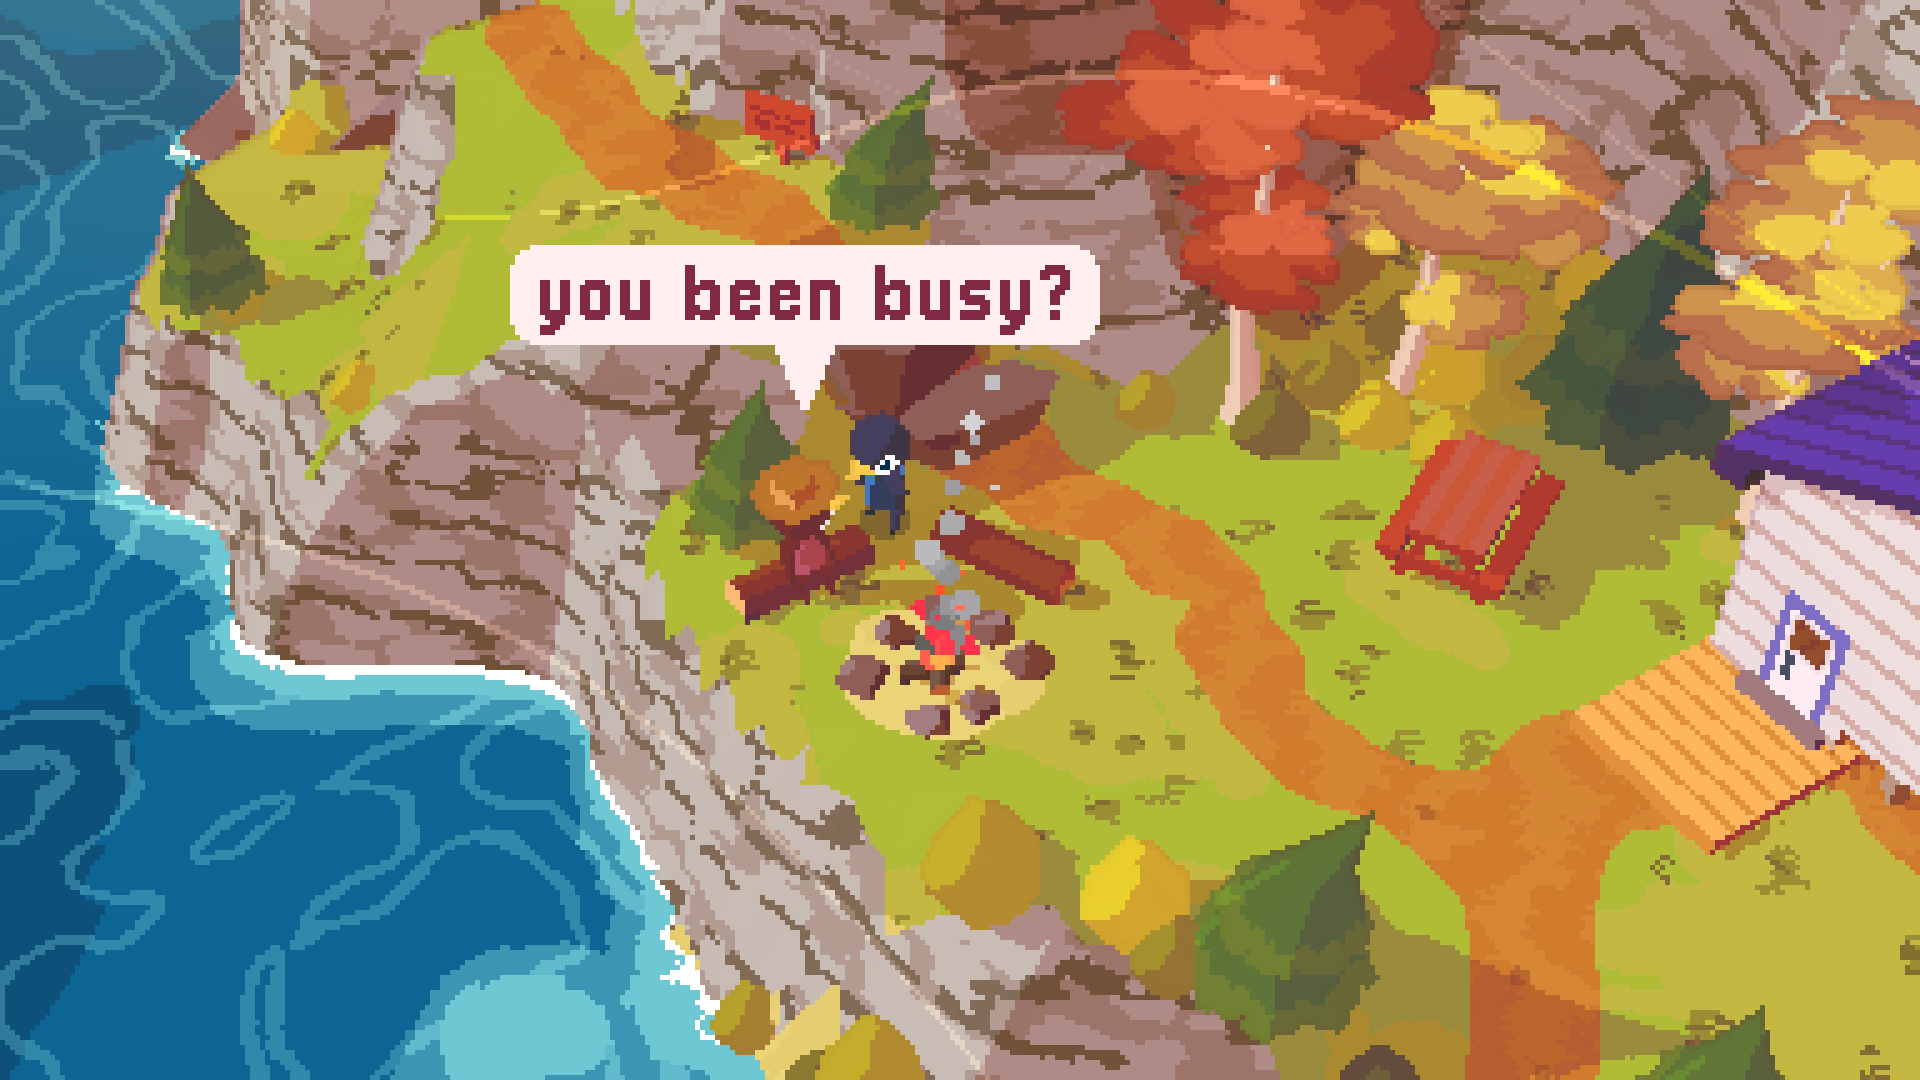
\includegraphics[width = 0.5\textwidth]{Imagenes/OCR/Pixel.png}
		\caption{Ejemplo imagen PixelArt }
	\end{figure}
	\item Texto en bocadillos.
		\begin{figure}[H]
		\centering
		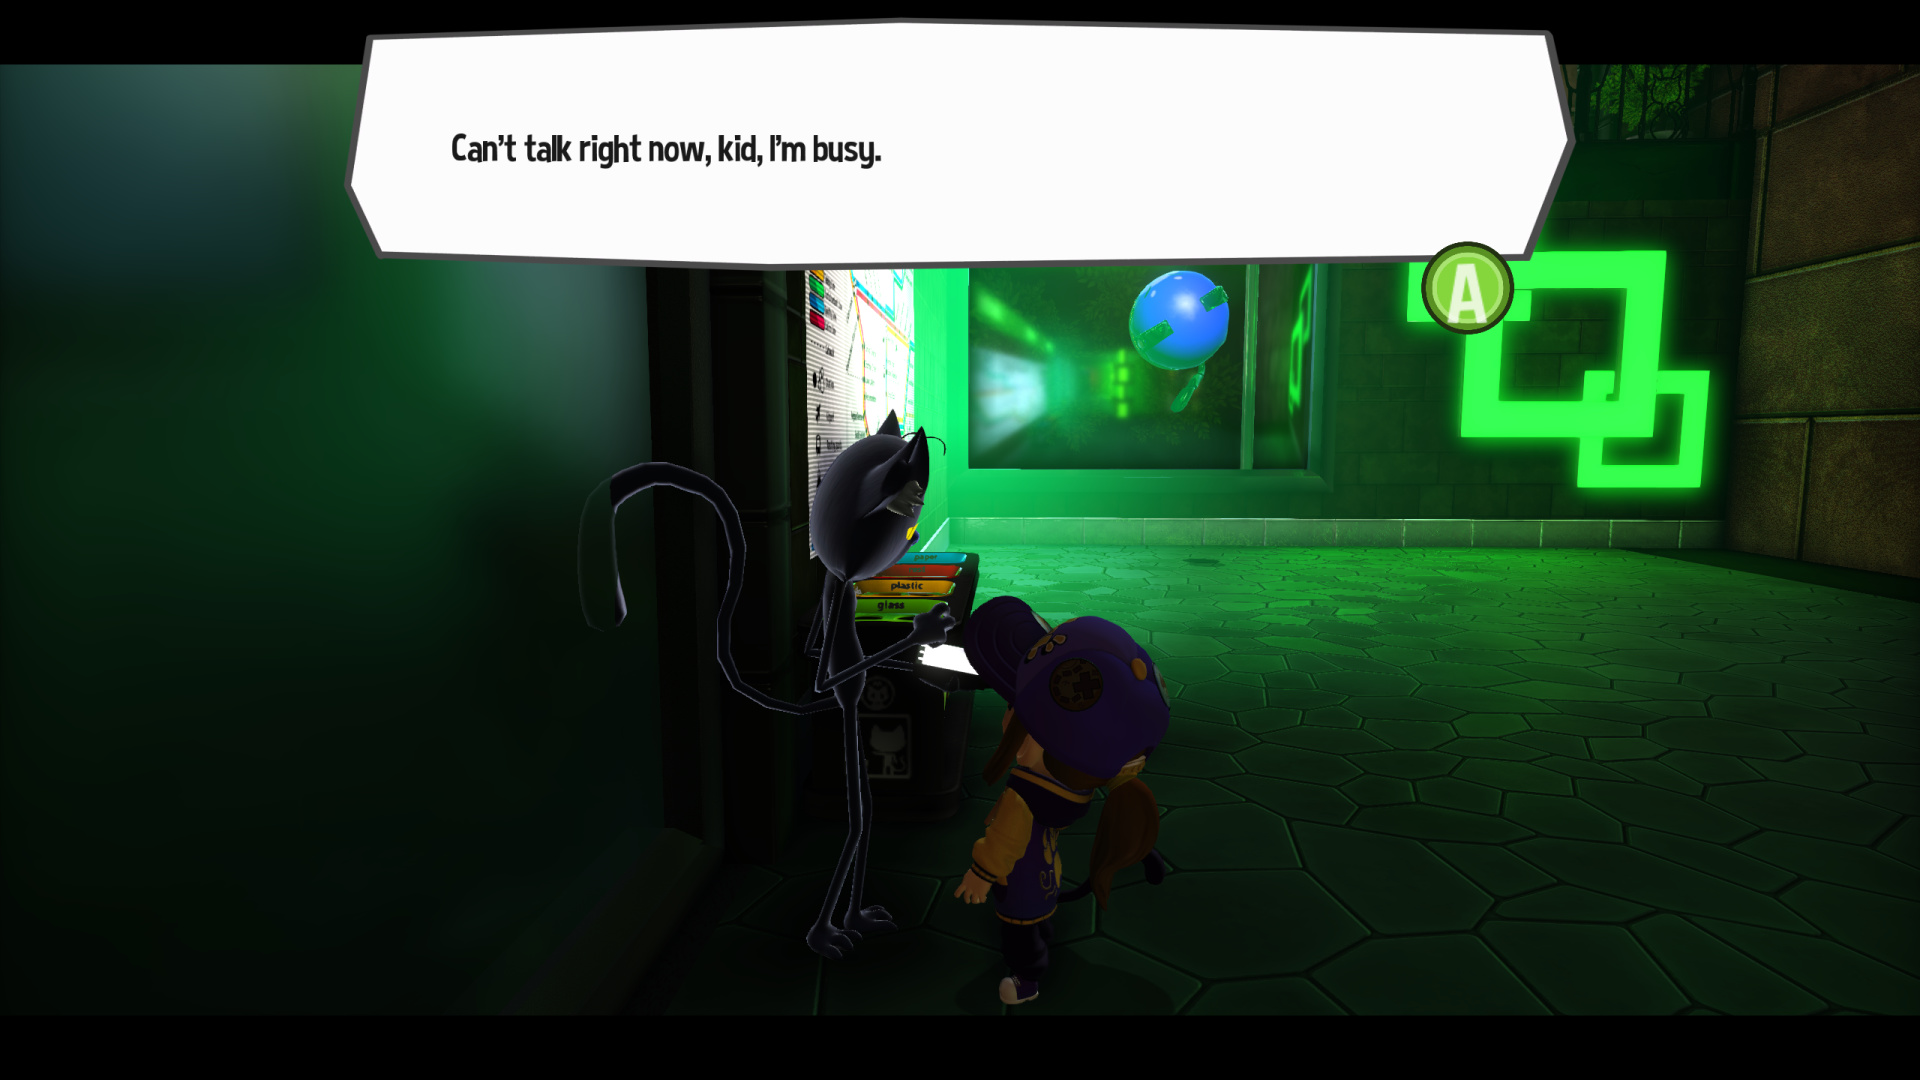
\includegraphics[width = 0.5\textwidth]{Imagenes/OCR/Boc.png}
		\caption{Ejemplo imagen de texto en bocadillo }
	\end{figure}
	\item Texto en bocadillos con poca diferenciación con el fondo.
		\begin{figure}[H]
		\centering
		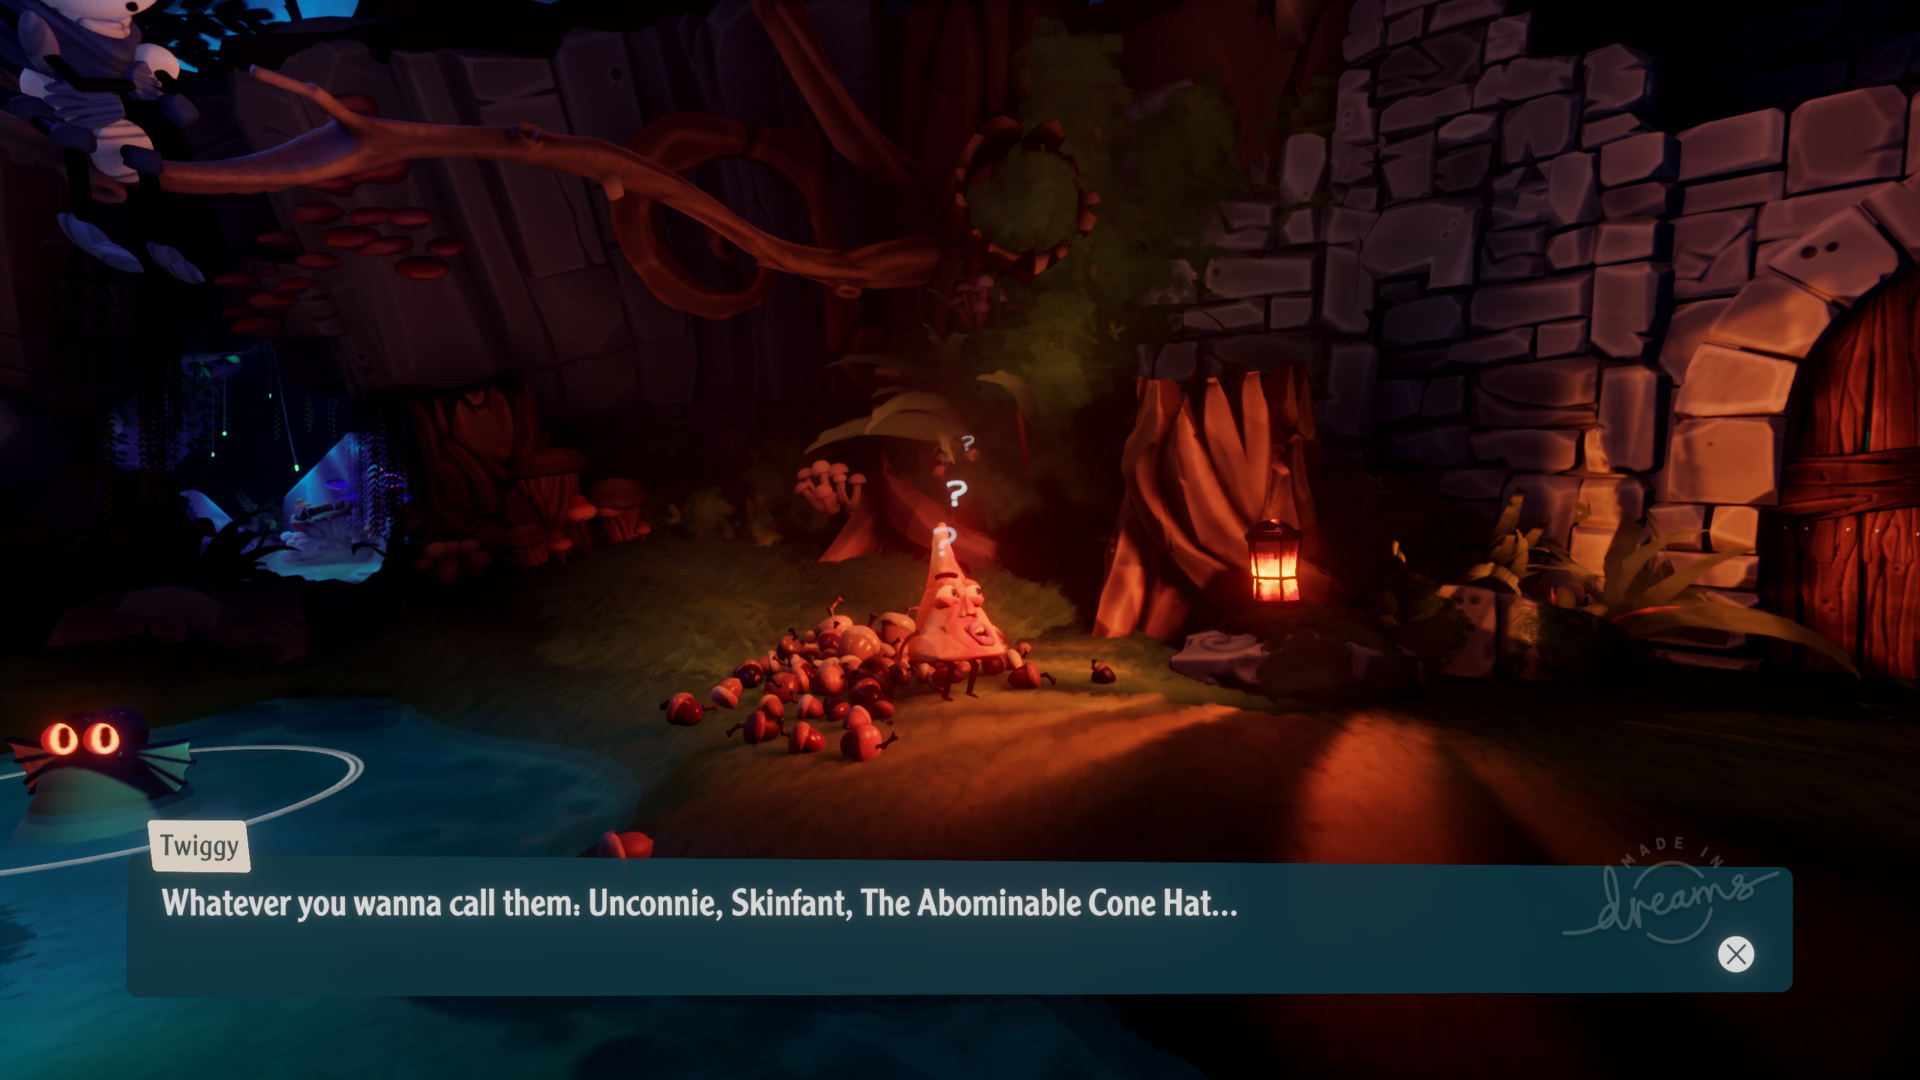
\includegraphics[width = 0.5\textwidth]{Imagenes/OCR/Boc2.png}
		\caption{Ejemplo imagen de texto en bocadillos con poca diferenciación con el fondo }
	\end{figure}
\end{enumerate} 

\subsection{Preprocesamiento de imágenes}
\footnote{(Image Processing in OpenCV)\url {https://docs.opencv.org/4.x/d2/d96/tutorial_py_table_of_contents_imgproc.html}}
El preprocesamiento de imágenes consiste en aplicar técnicas que modifican las imágenes para que sea más fácil de reconocer por una OCR el texto existente.
Para saber que técnicas mejora el reconocimiento y baja el CER, se ha ido probando con cada una de ellas, obteniendo los resultados e identificando aquellas técnicas que ayuda a mejorar el CER medio.
Las técnicas probadas son las siguientes:

\begin{enumerate}
	\item Escala de grises:
	Convierte una imagen a un formato de un solo canal, representando solo la intensidad de luz. Es útil para simplificar y reducir la cantidad de datos cuando el color no es relevante.
	\begin{figure}[H]
		\centering
		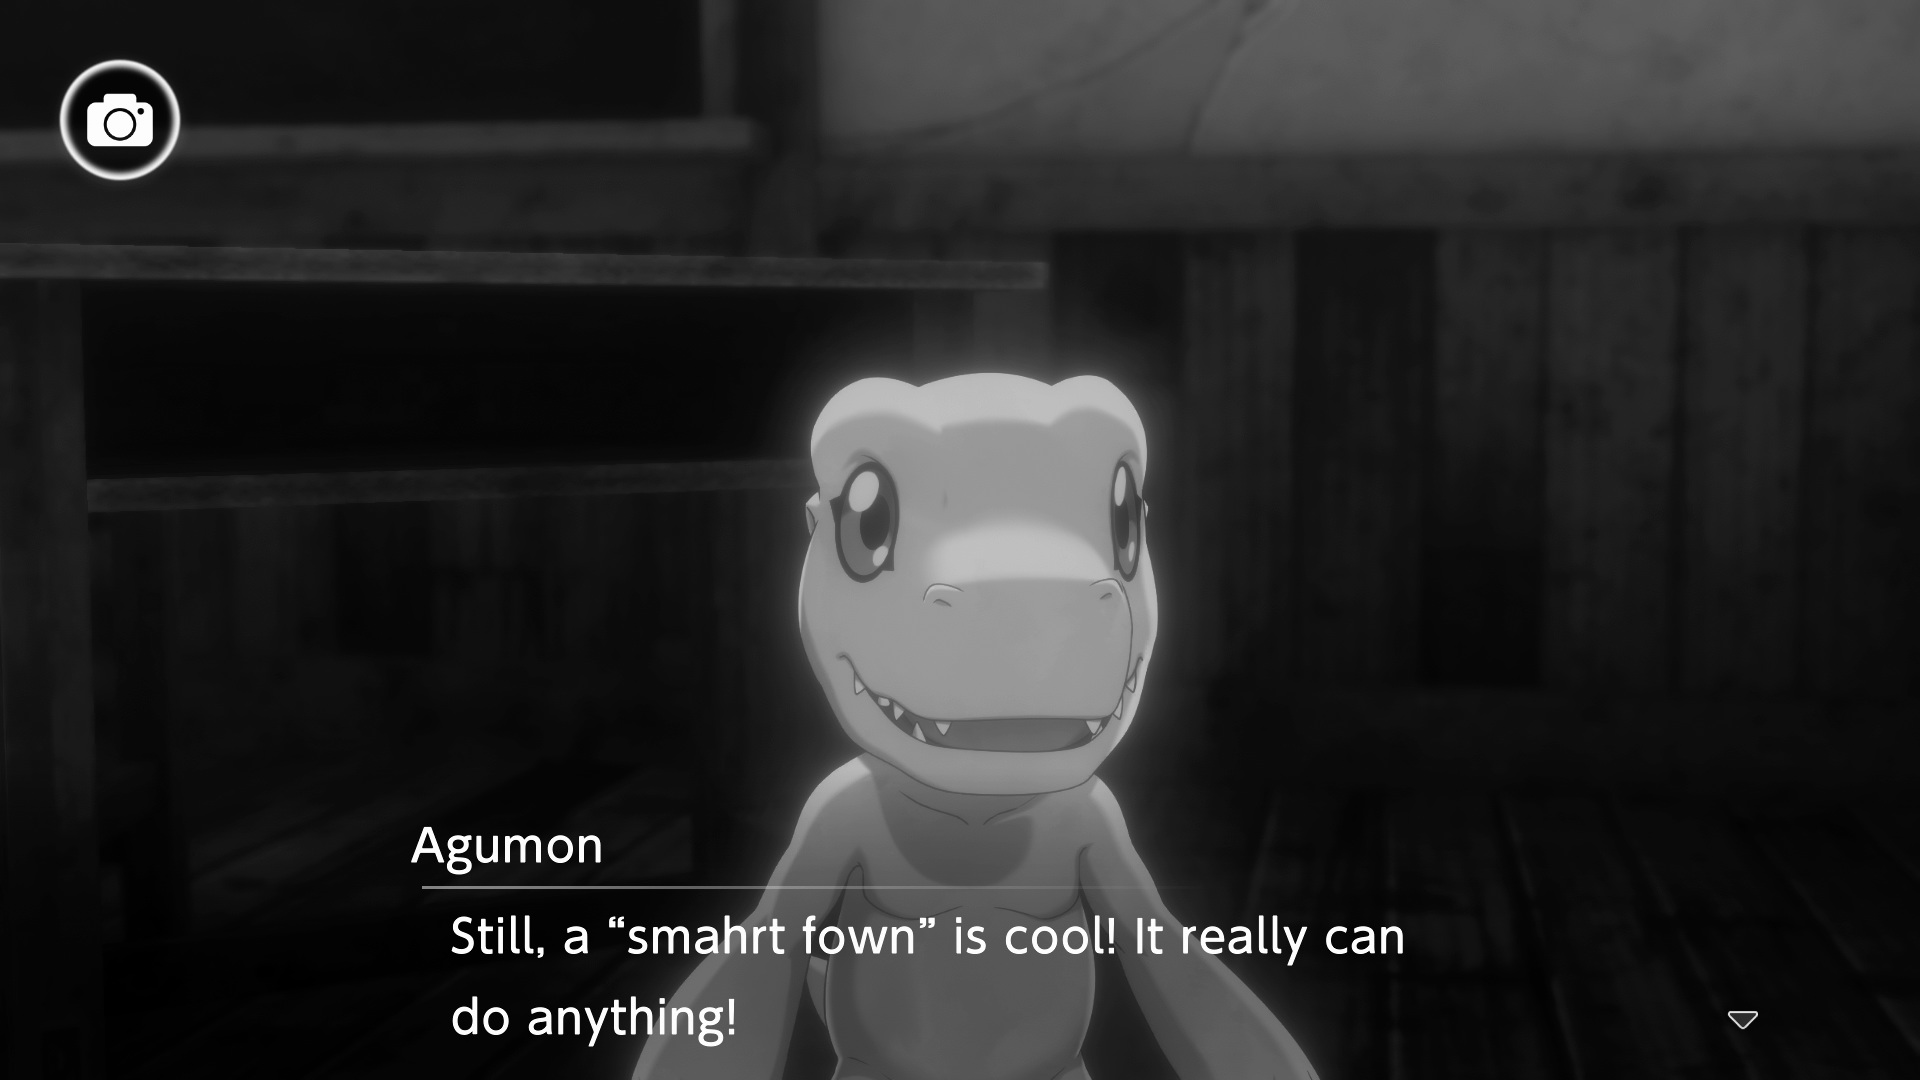
\includegraphics[width = 0.5\textwidth]{Imagenes/Preprocesado/1.png}
	\end{figure}
	\item Aumentar contraste: 
	Mejora la diferencia entre las áreas claras y oscuras en una imagen, lo que facilita la detección de detalles.
		\begin{figure}[H]
		\centering
		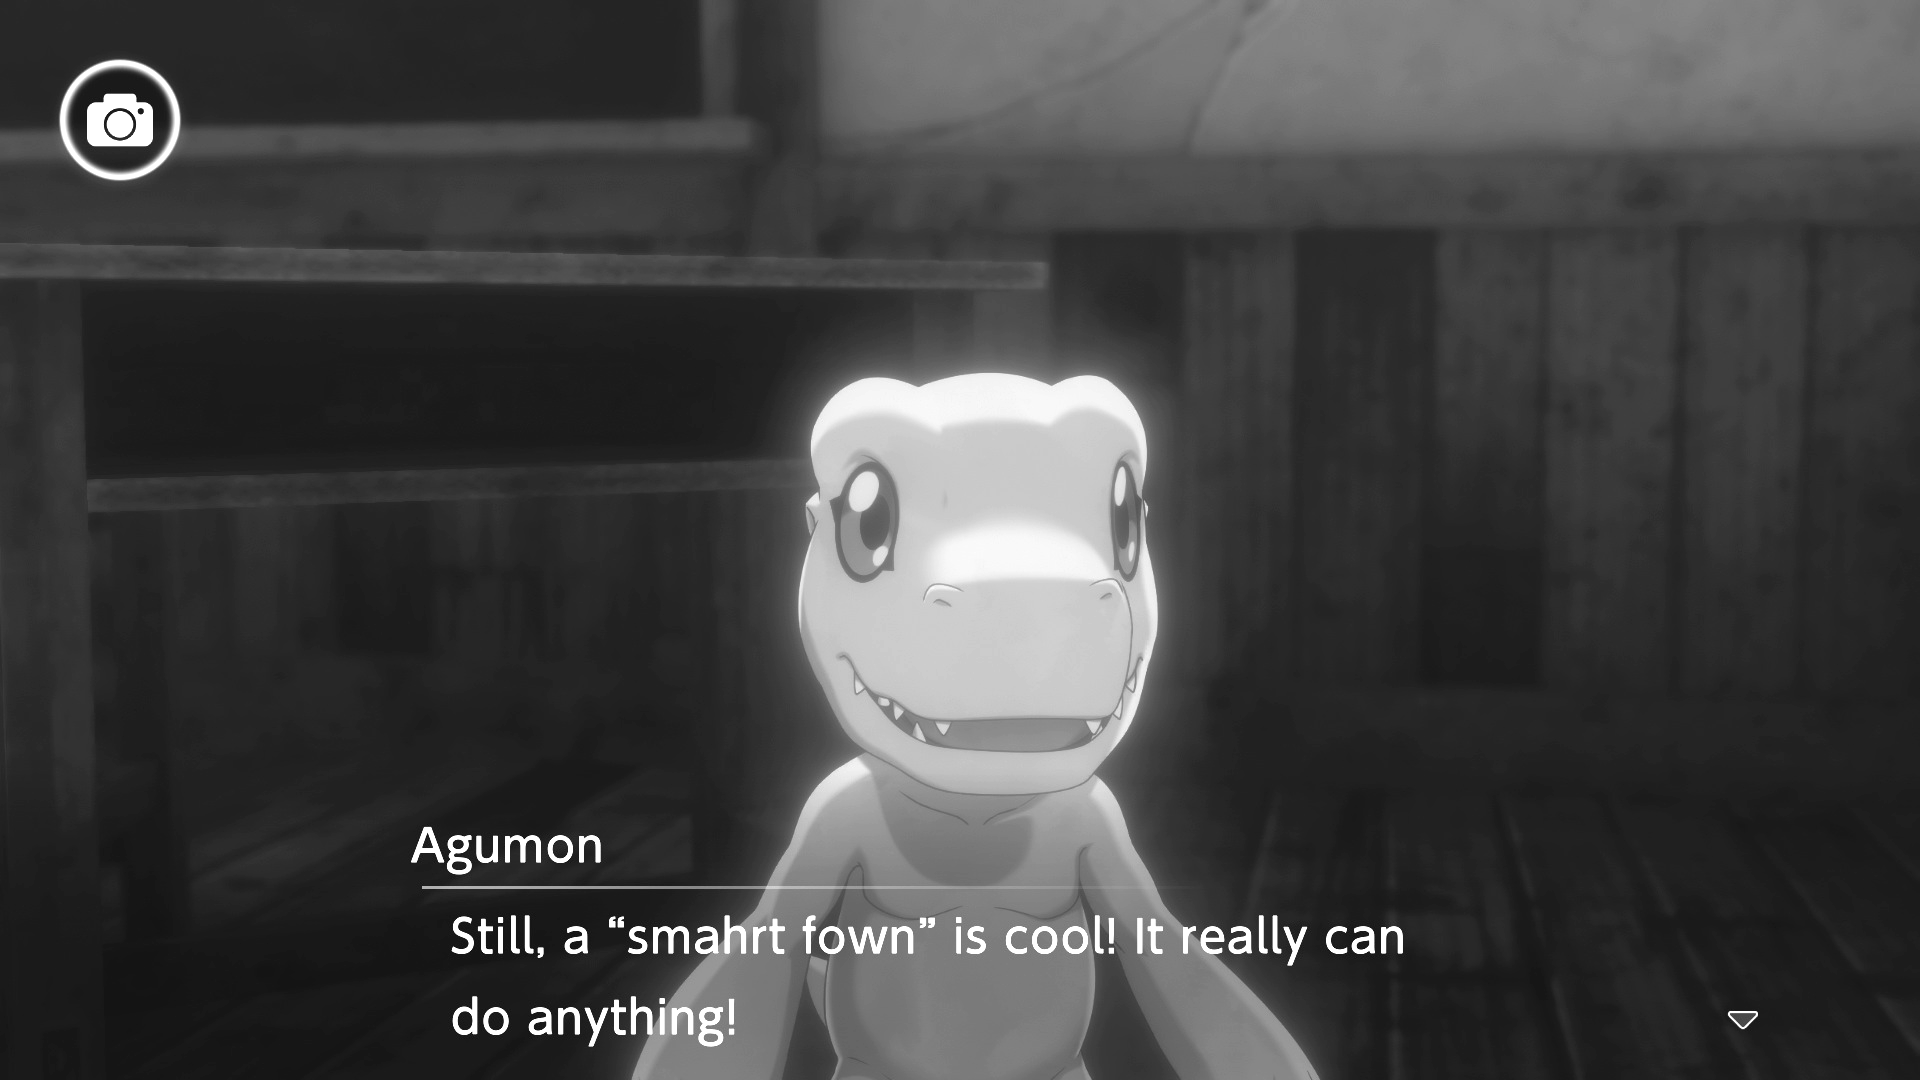
\includegraphics[width = 0.5\textwidth]{Imagenes/Preprocesado/2.png}
	\end{figure}
	\item Ecualización del histograma:
	Ajusta el contraste de la imagen extendiendo la distribución de los niveles de gris, mejorando el rango dinámico y resaltando los detalles.
		\begin{figure}[H]
		\centering
		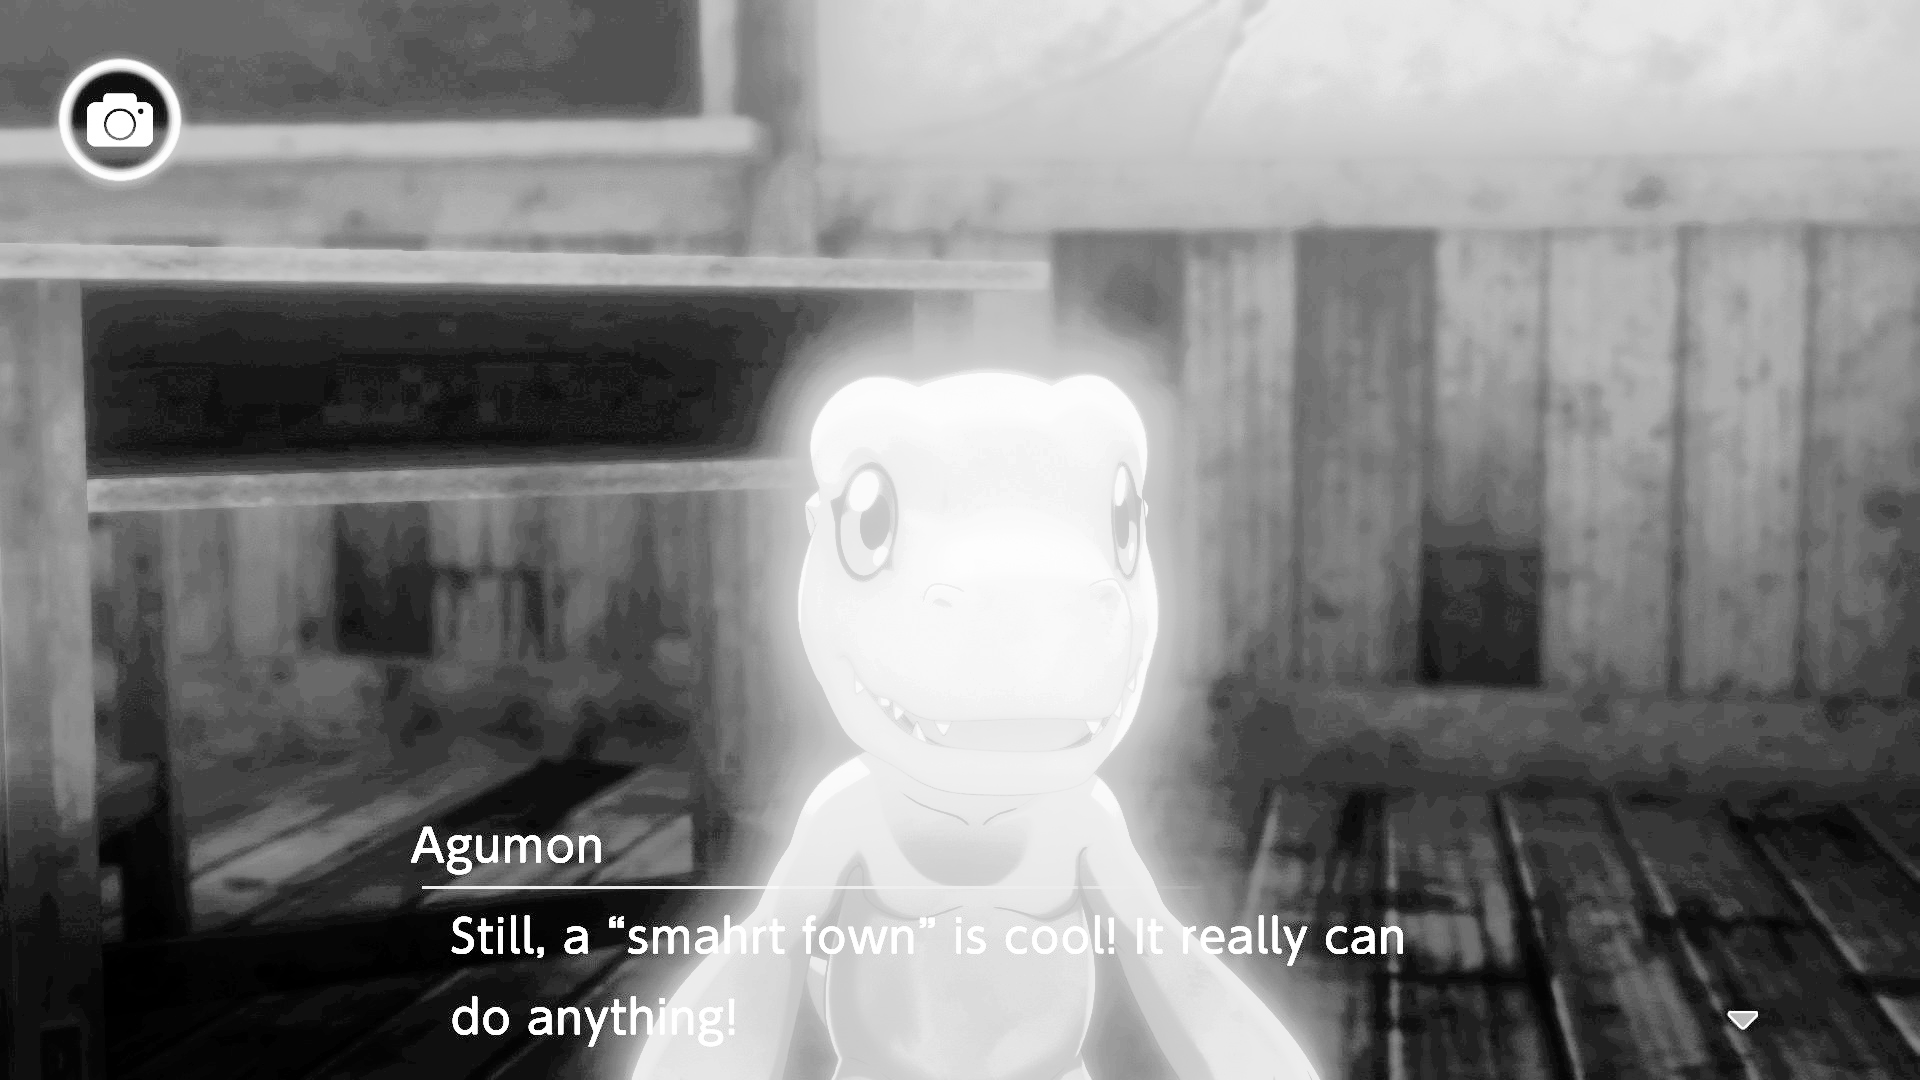
\includegraphics[width = 0.5\textwidth]{Imagenes/Preprocesado/3.png}
	\end{figure}
	
	\item Corrección del gamma:
	Ajusta los valores de intensidad en la imagen para compensar la percepción humana y los errores del sensor, lo que puede hacer que ciertas áreas sean más visibles.
		\begin{figure}[H]
		\centering
		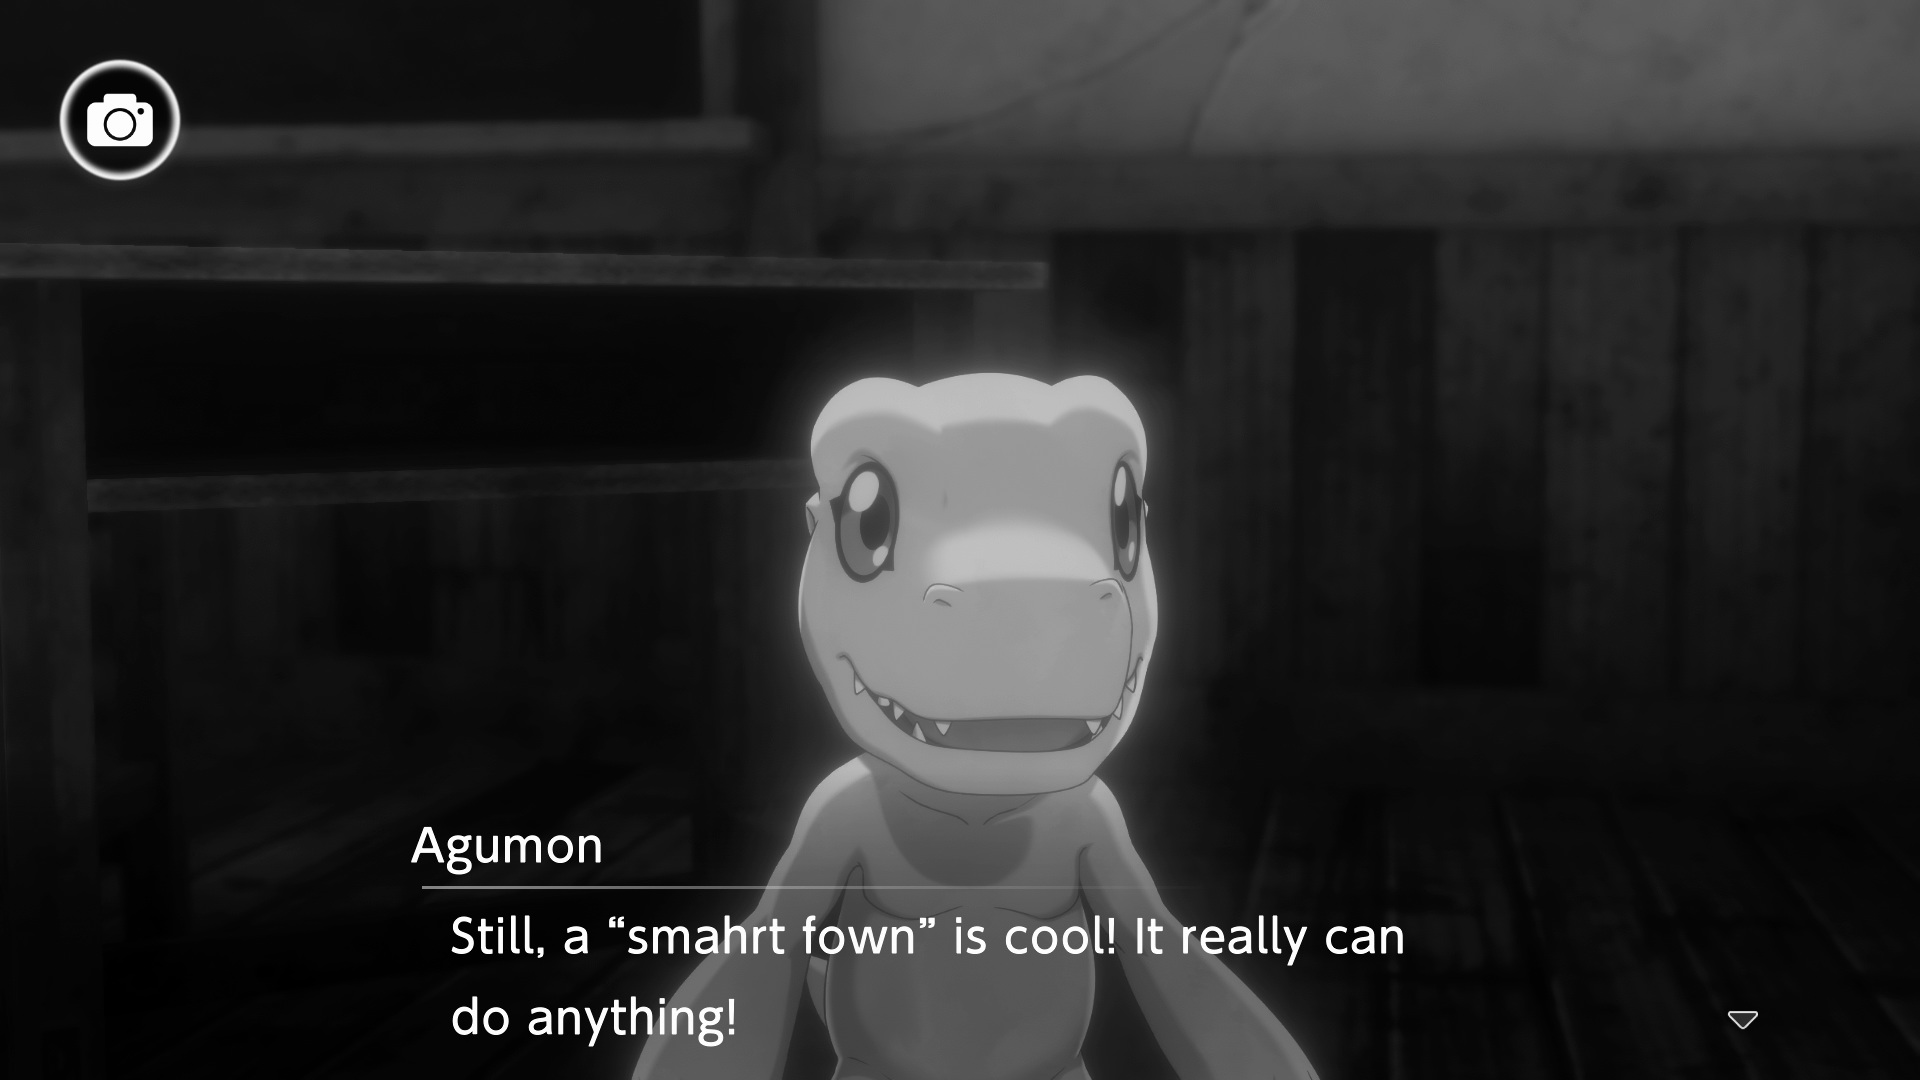
\includegraphics[width = 0.5\textwidth]{Imagenes/Preprocesado/4.png}
	\end{figure}
	
	\item Filtro de nitidez: 
	Realza los bordes de una imagen para destacar detalles, útil en aplicaciones donde se requiere mayor definición.
		\begin{figure}[H]
		\centering
		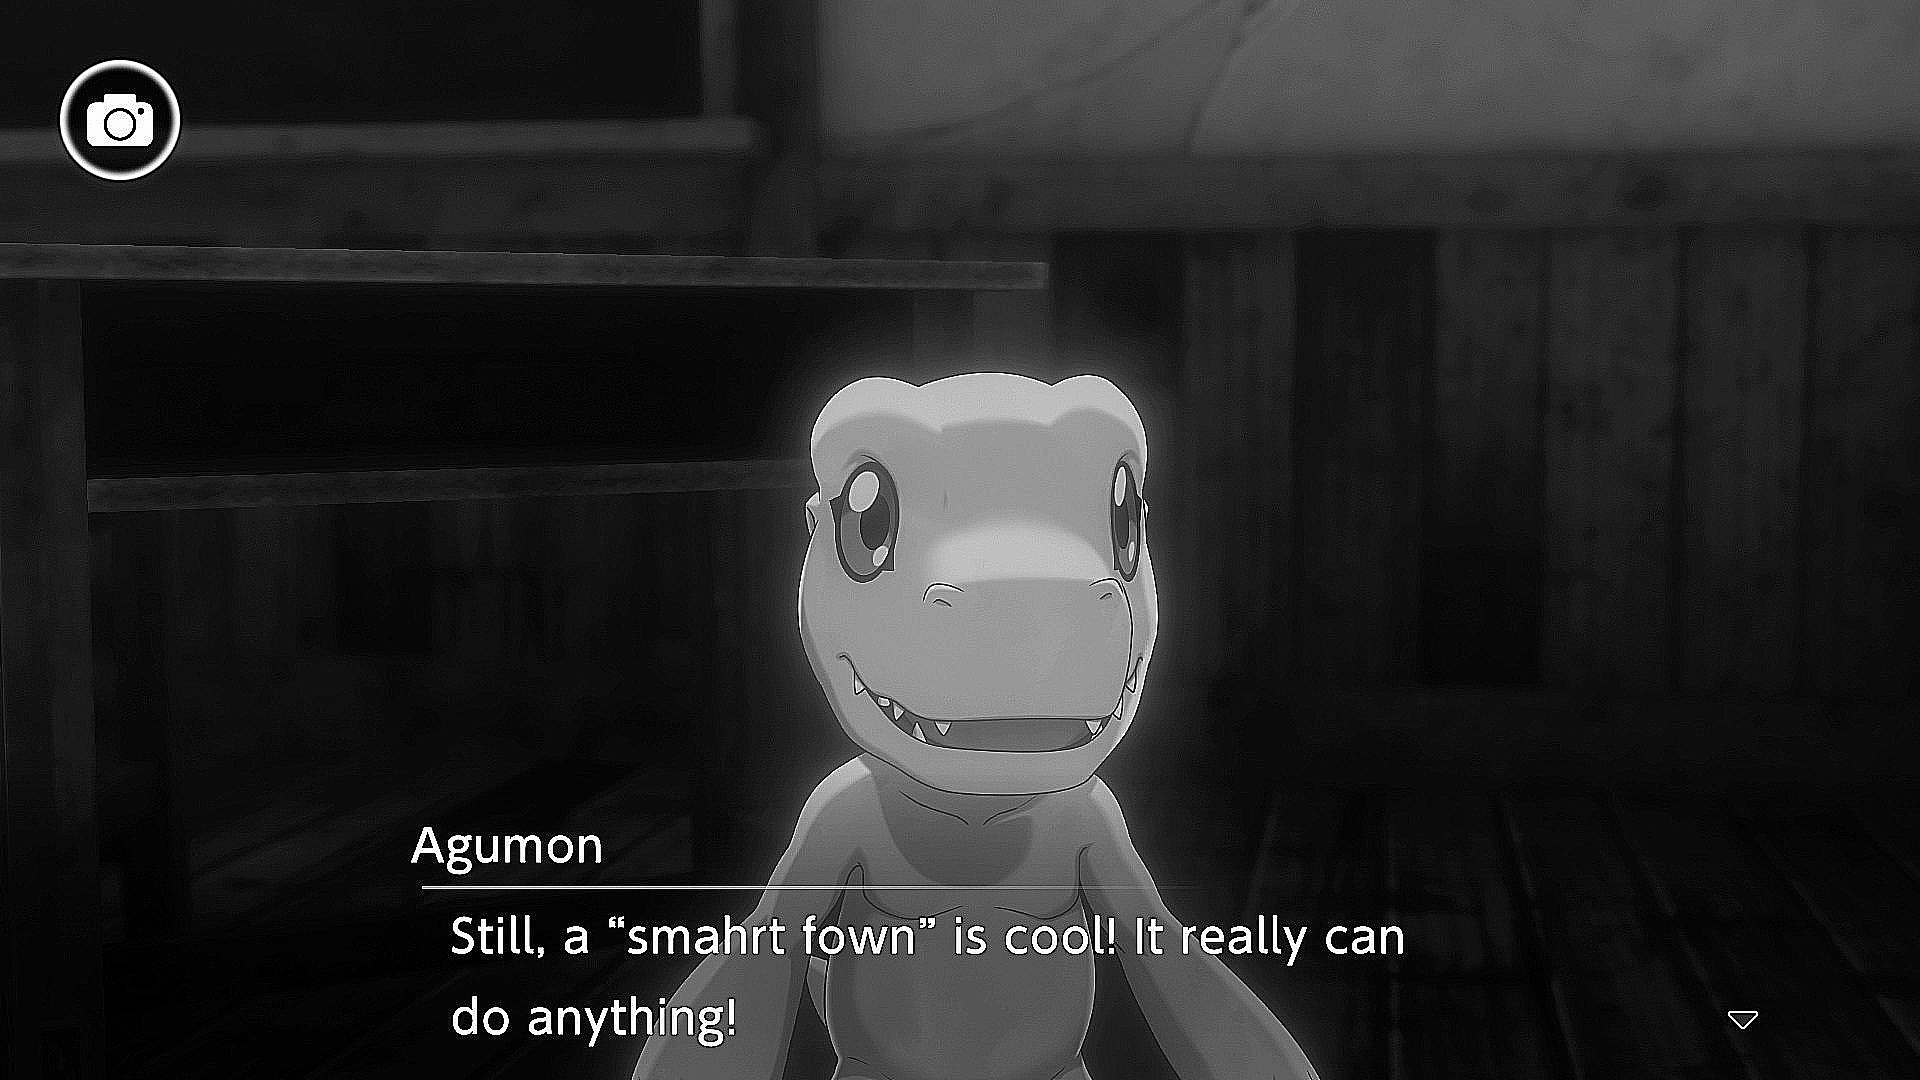
\includegraphics[width = 0.5\textwidth]{Imagenes/Preprocesado/5.png}
	\end{figure}
	
	\item Adaptive Thresholding:
	Segmenta una imagen dividiéndola en áreas claras y oscuras, aplicando un umbral que se ajusta de forma adaptativa a las variaciones locales de luz.
		\begin{figure}[H]
		\centering
		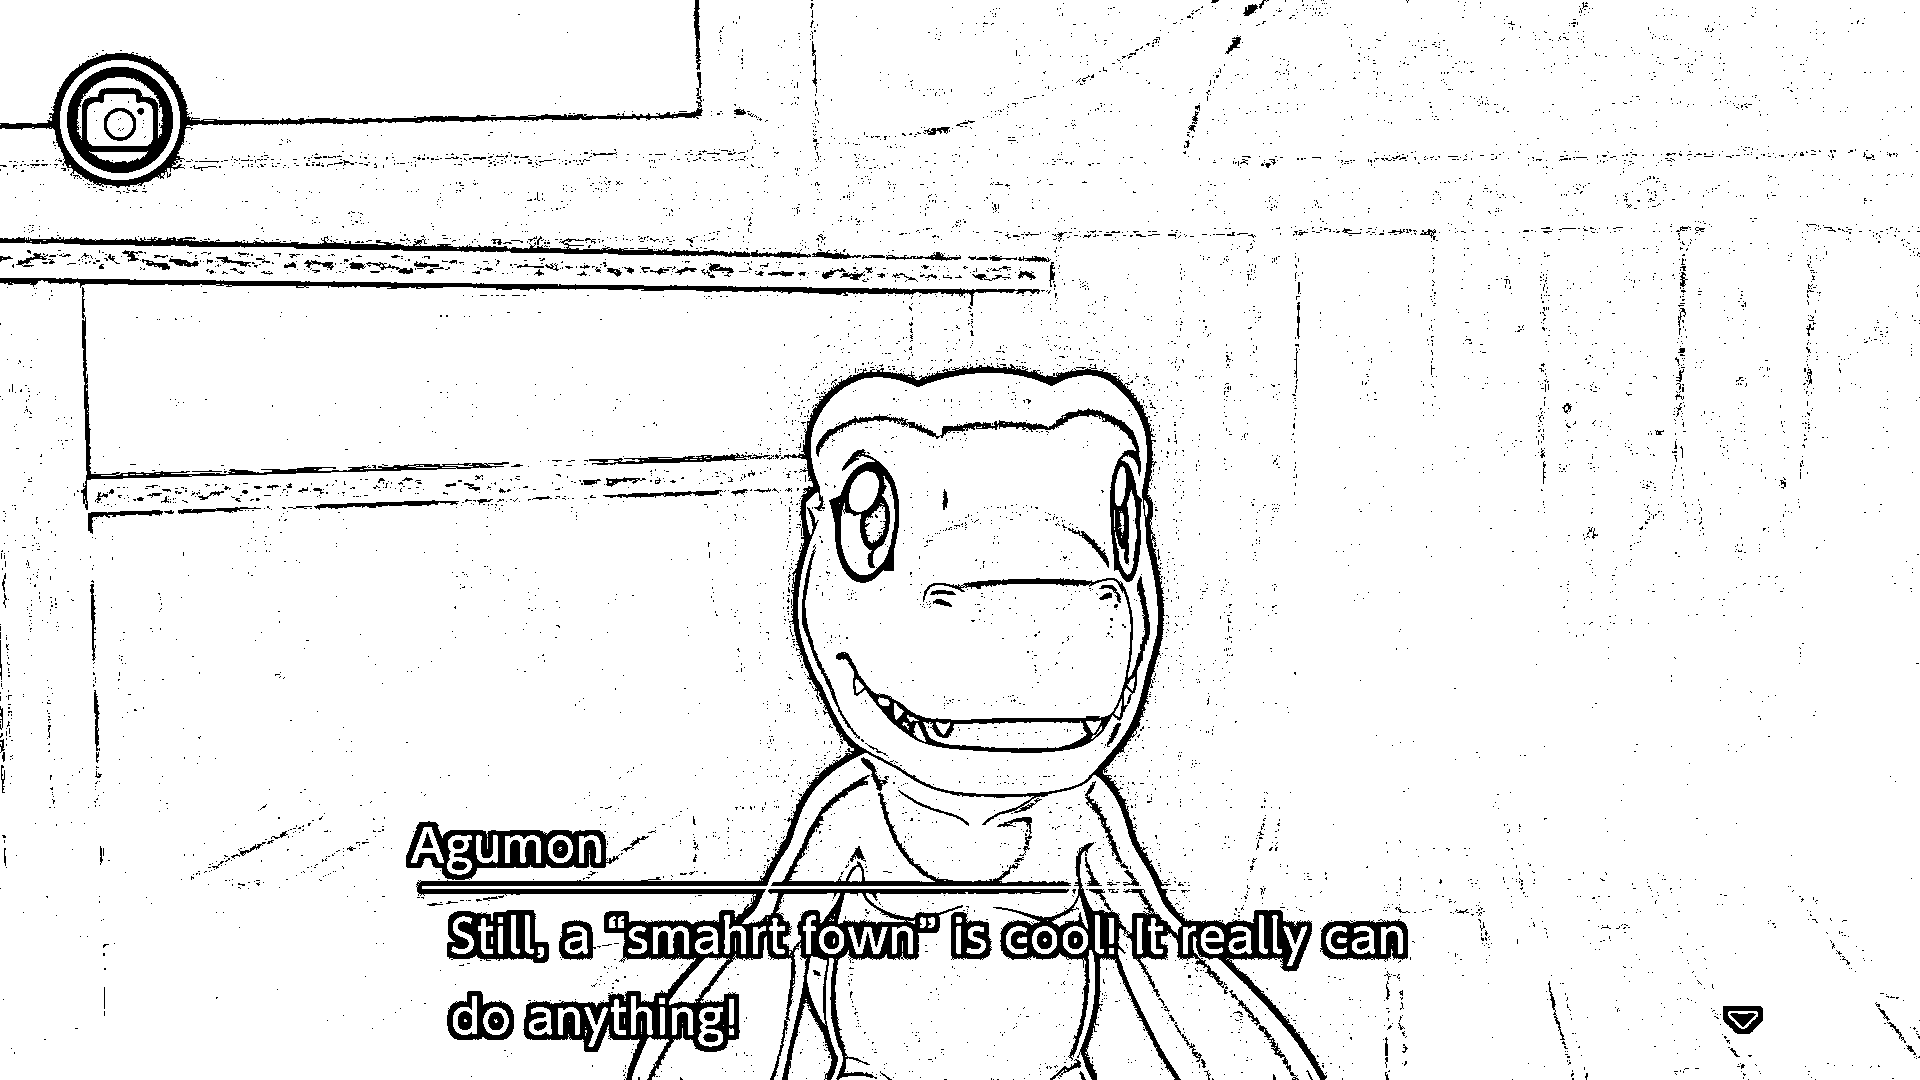
\includegraphics[width = 0.5\textwidth]{Imagenes/Preprocesado/6.png}
	\end{figure}
	
	\item Simple Thresholding: 
	Asigna un valor binario a cada píxel dependiendo de si está por encima o por debajo de un umbral específico, útil para crear máscaras y segmentación sencilla.
		\begin{figure}[H]
		\centering
		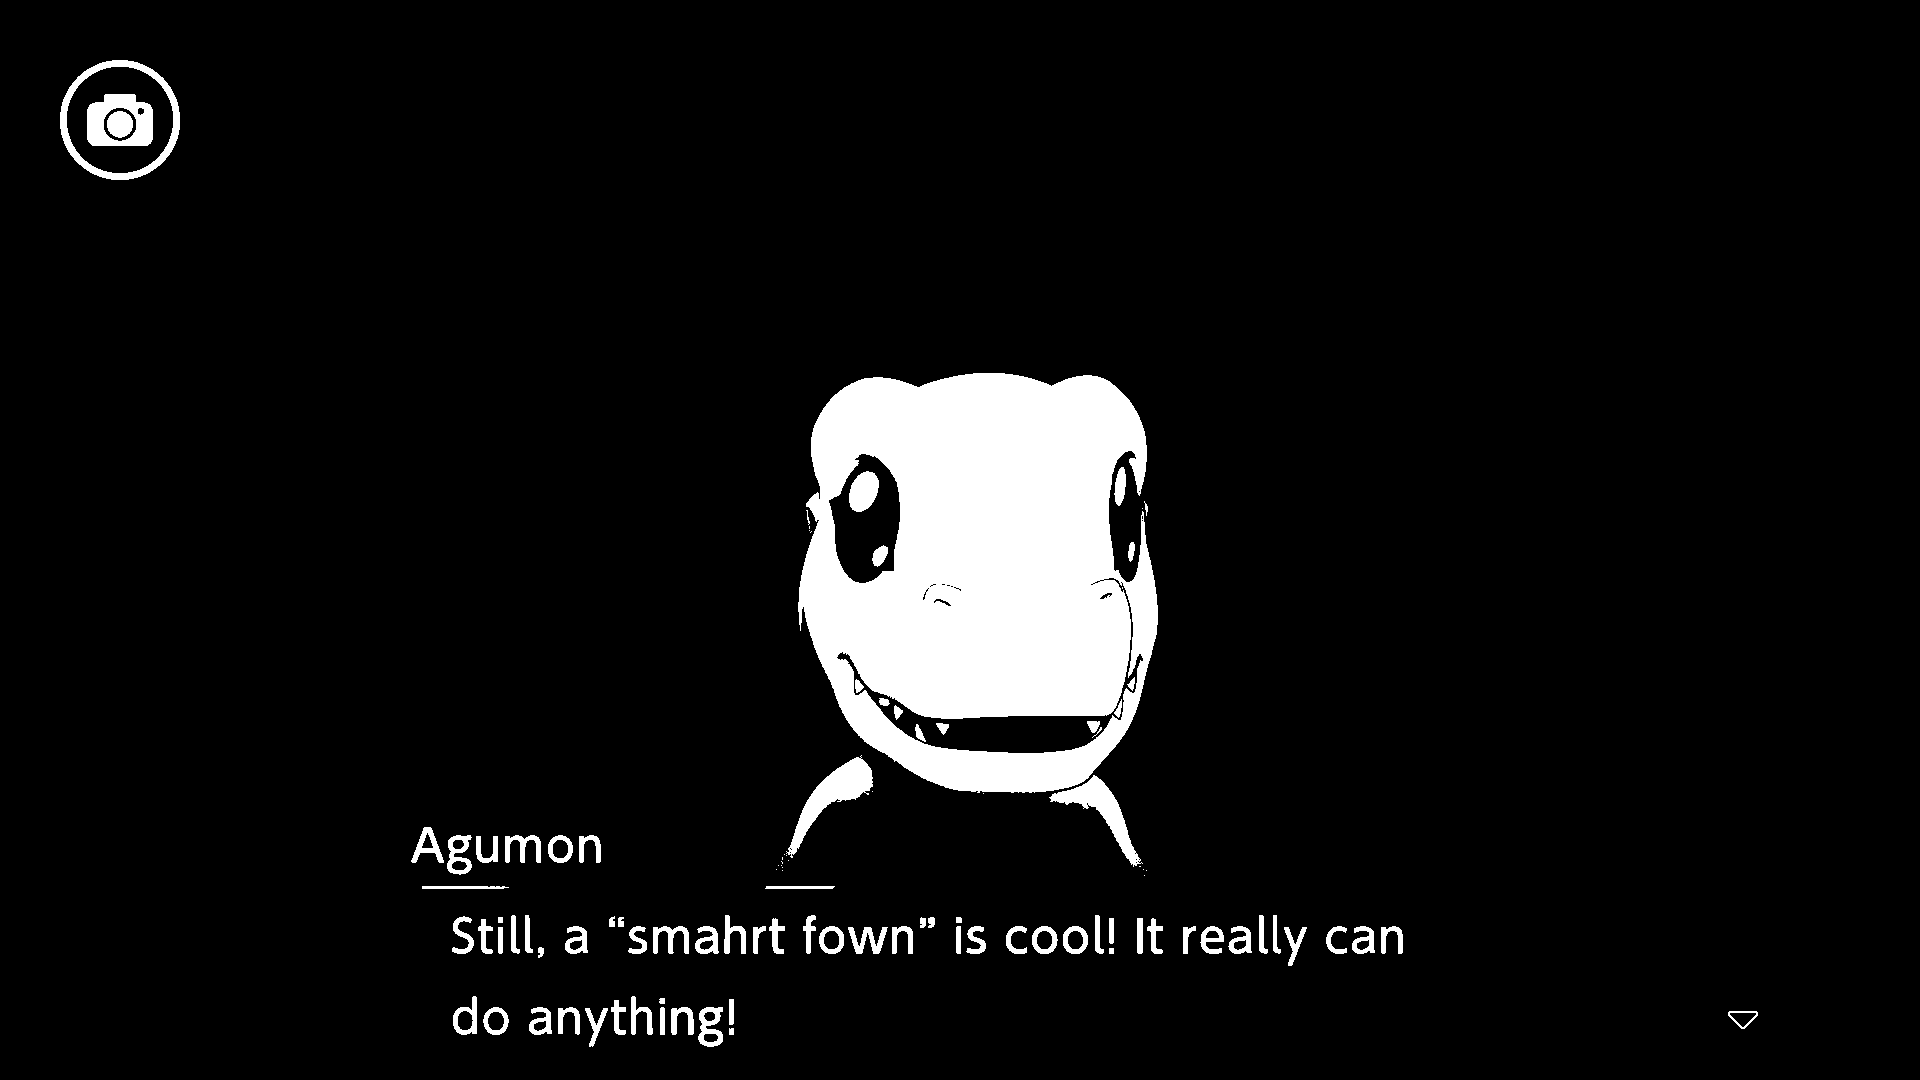
\includegraphics[width = 0.5\textwidth]{Imagenes/Preprocesado/7.png}
	\end{figure}
	
	\item Image Blurring (Desenfoque de Imagen): 
	Reduce el ruido y los detalles mediante técnicas como filtros Gaussianos o de promediado, comúnmente utilizado para suavizar imágenes antes de un análisis.
		\begin{figure}[H]
		\centering
		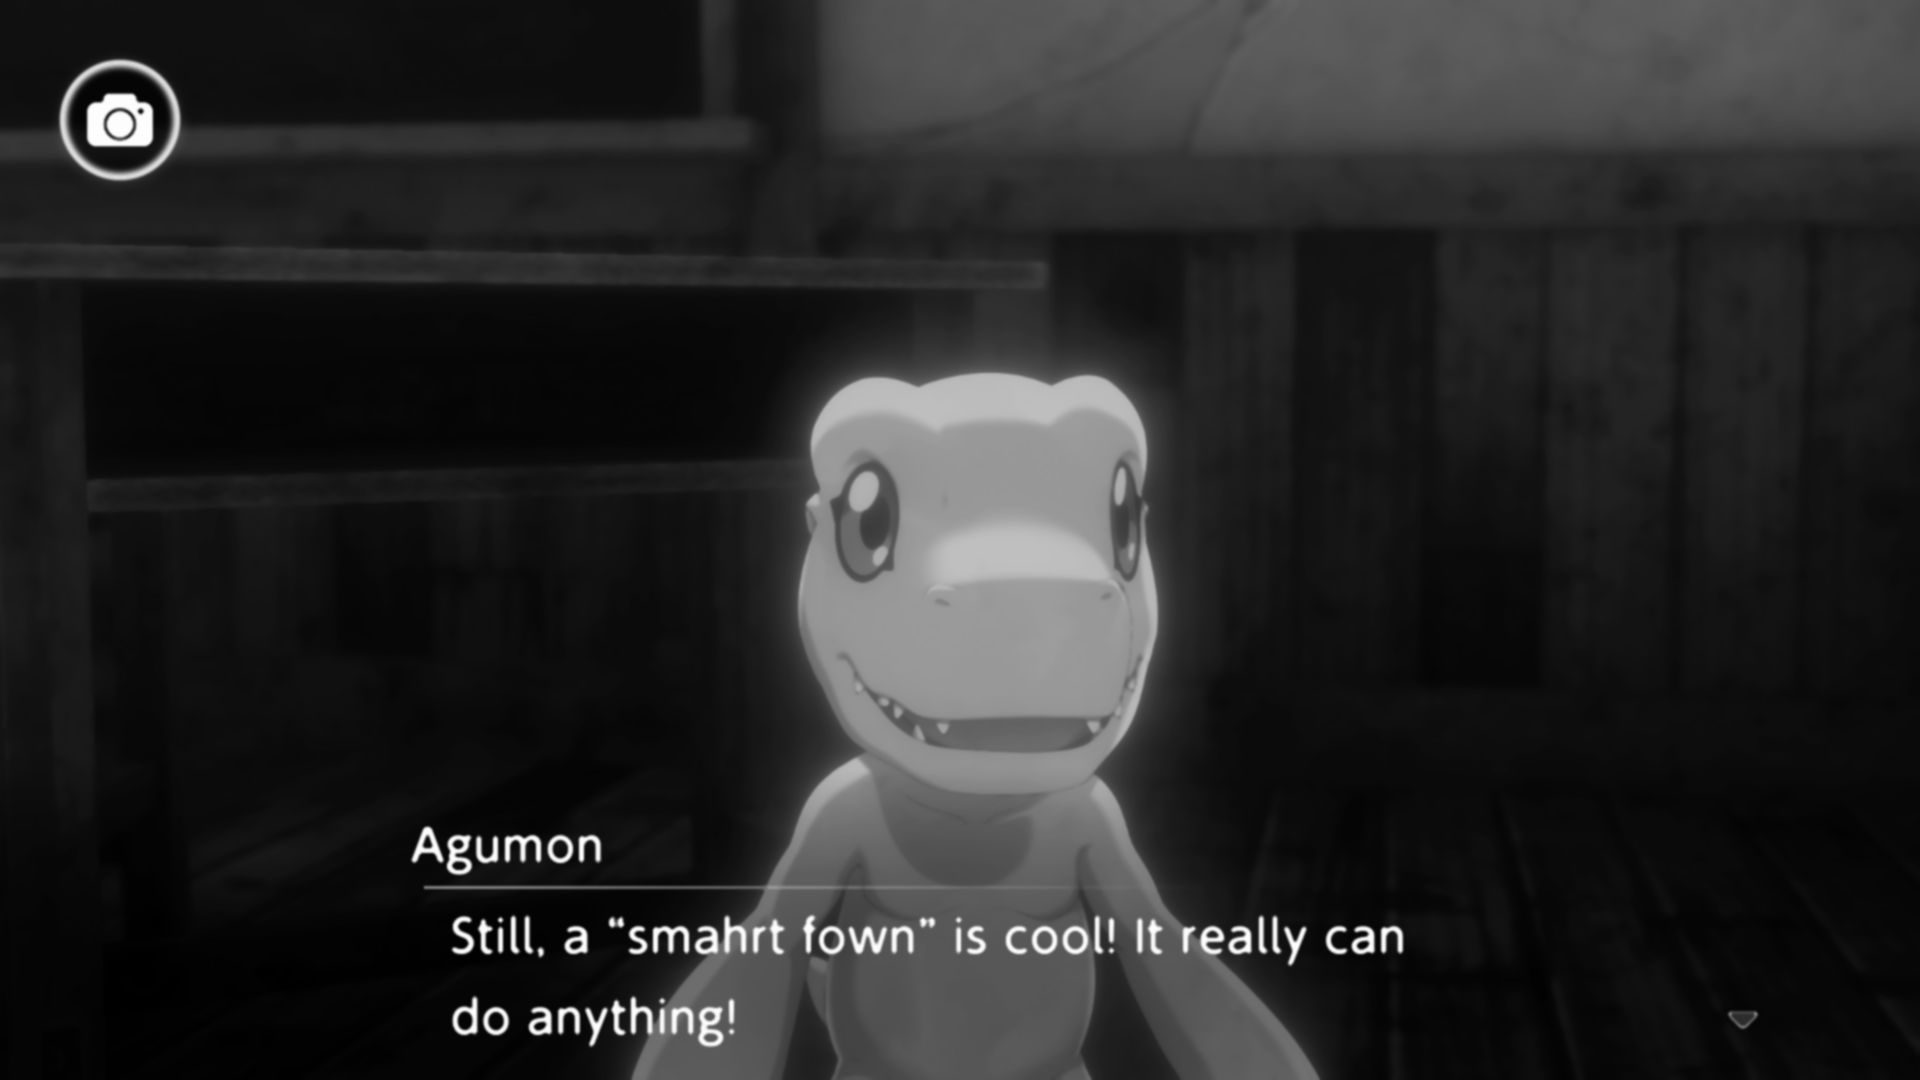
\includegraphics[width = 0.5\textwidth]{Imagenes/Preprocesado/8.png}
	\end{figure}
	
	\item Redimensionar la imagen: 
	Cambia las dimensiones de una imagen, lo que puede ser útil para normalizar entradas a una red neuronal o ajustar el tamaño de una imagen para procesamiento.
		\begin{figure}[H]
		\centering
		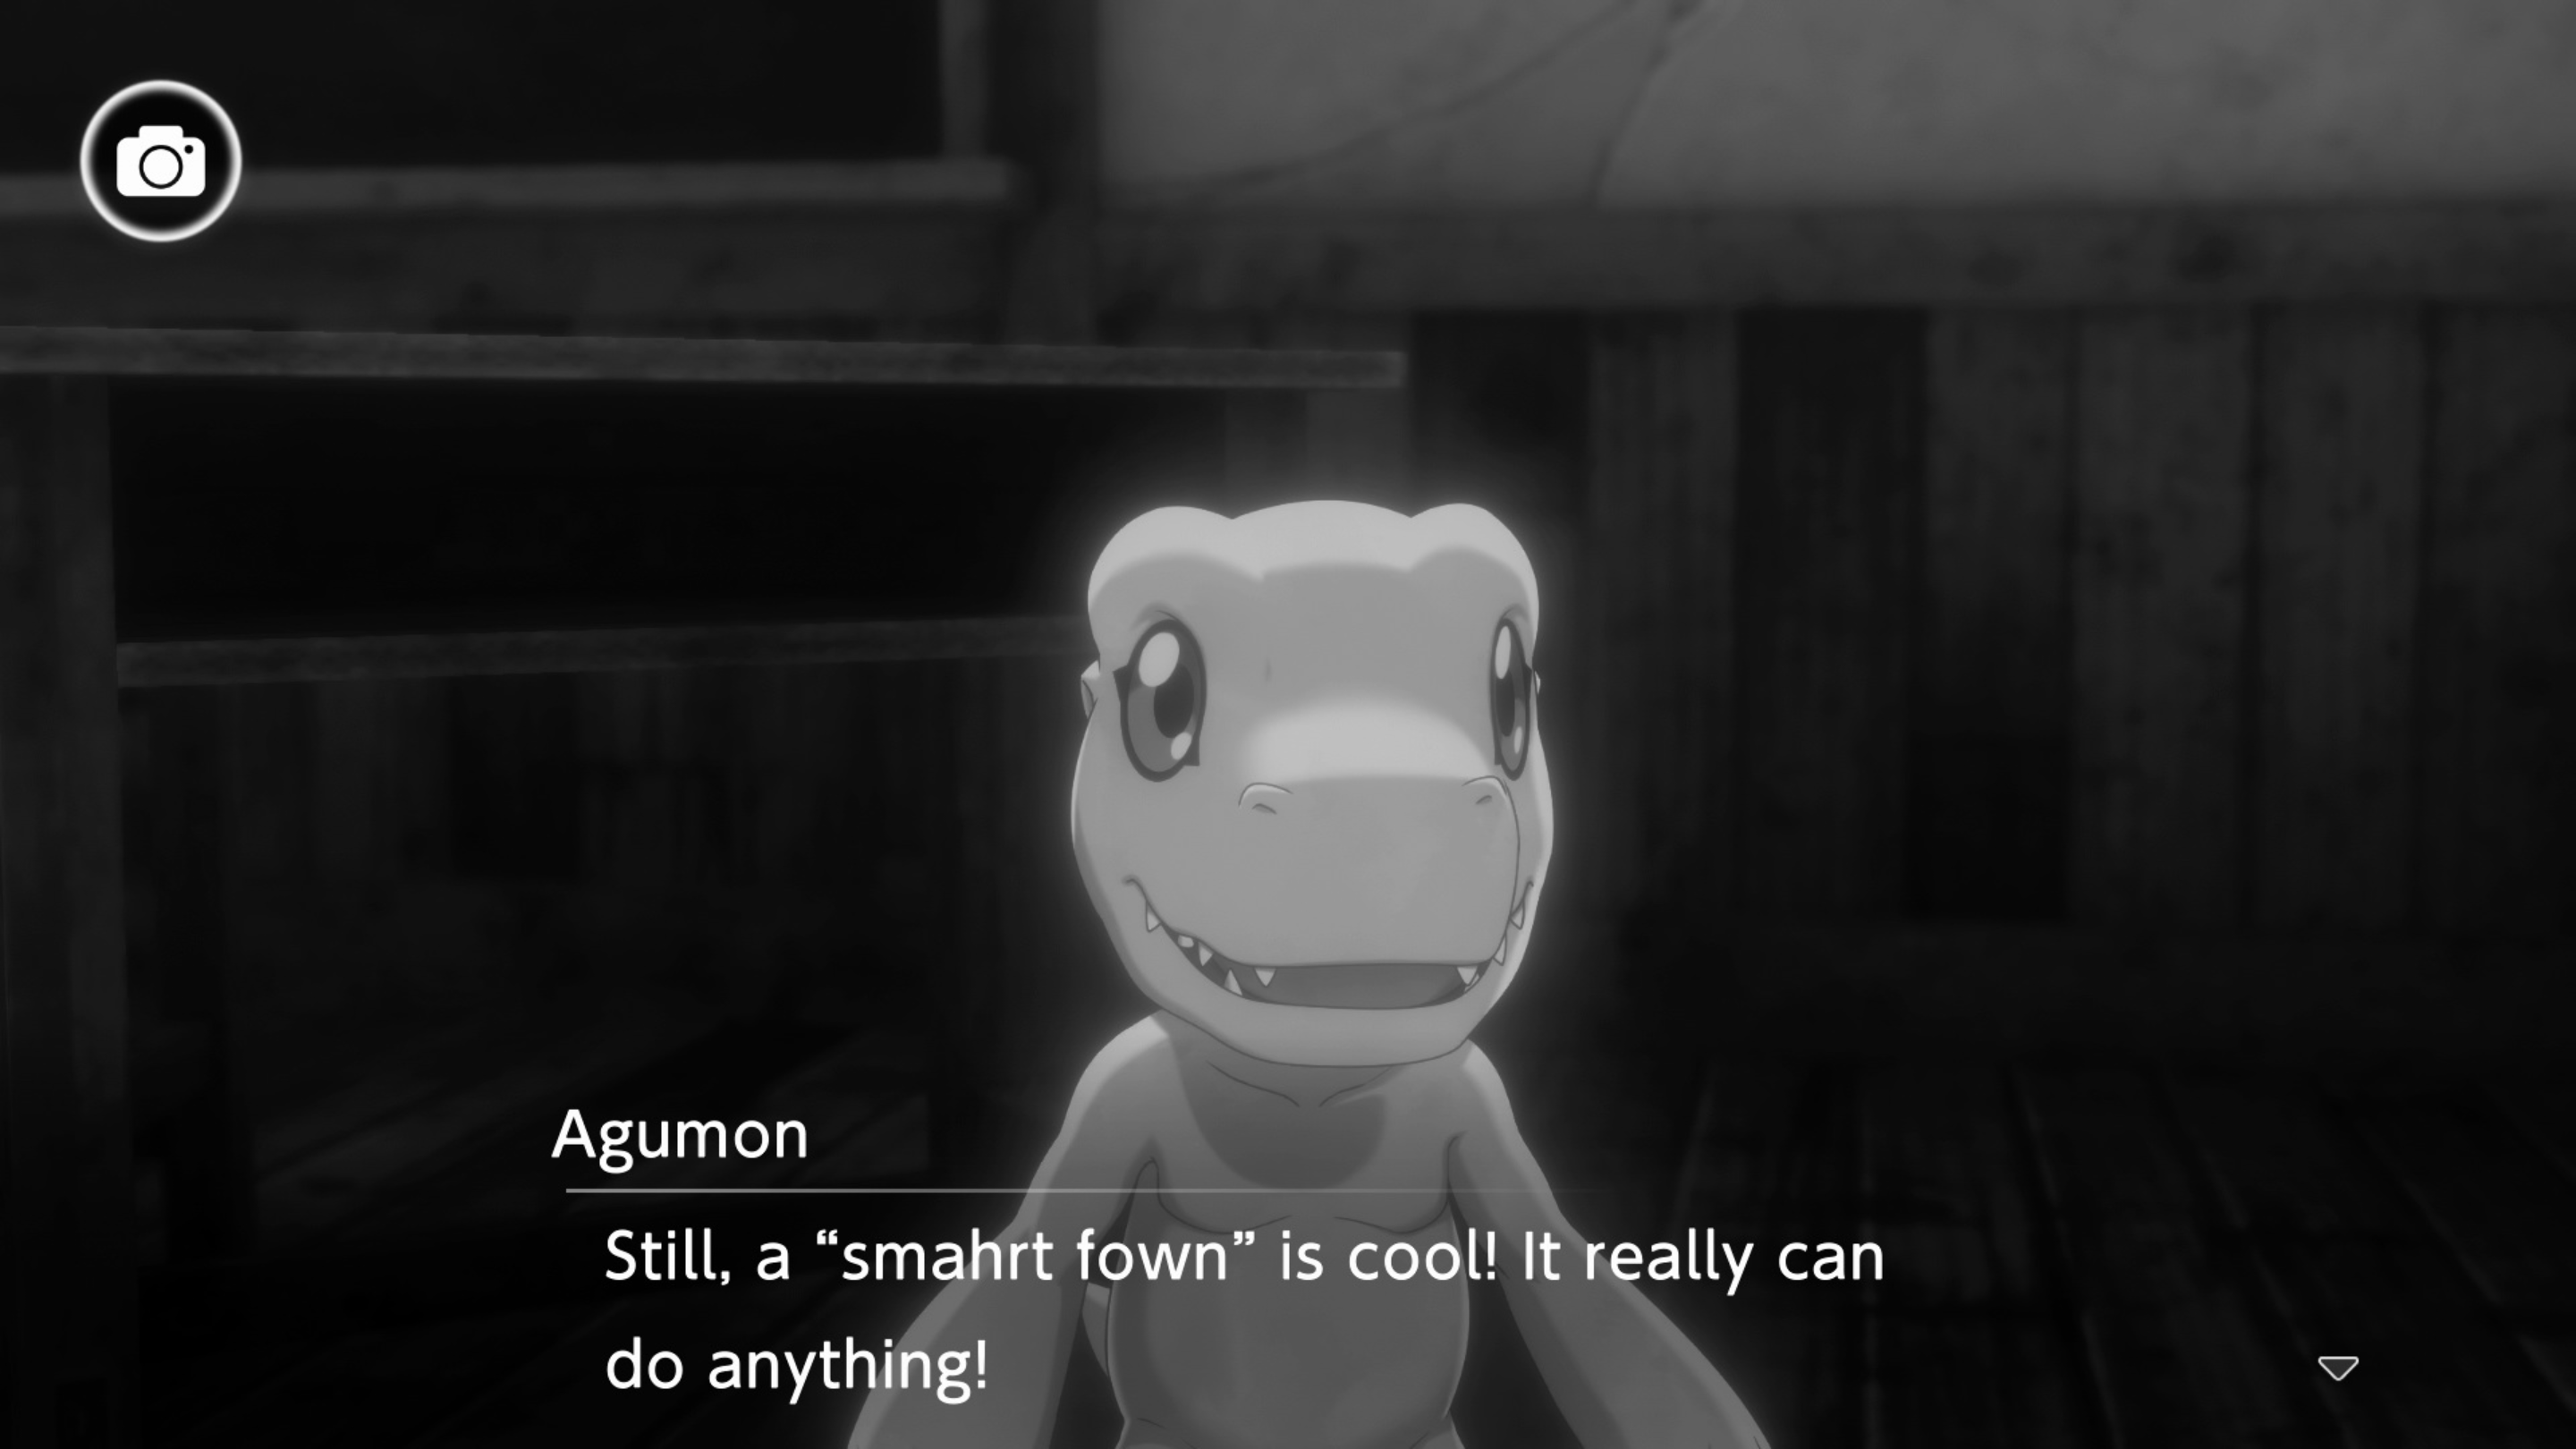
\includegraphics[width = 0.5\textwidth]{Imagenes/Preprocesado/9.png}
	\end{figure}
		
	\item Dilatar y erosionar: 
	Técnicas de morfología matemática que expanden o reducen las regiones blancas (o los objetos) en una imagen binaria, útiles para limpieza de ruido o cierre de contornos.
		\begin{figure}[H]
		\centering
		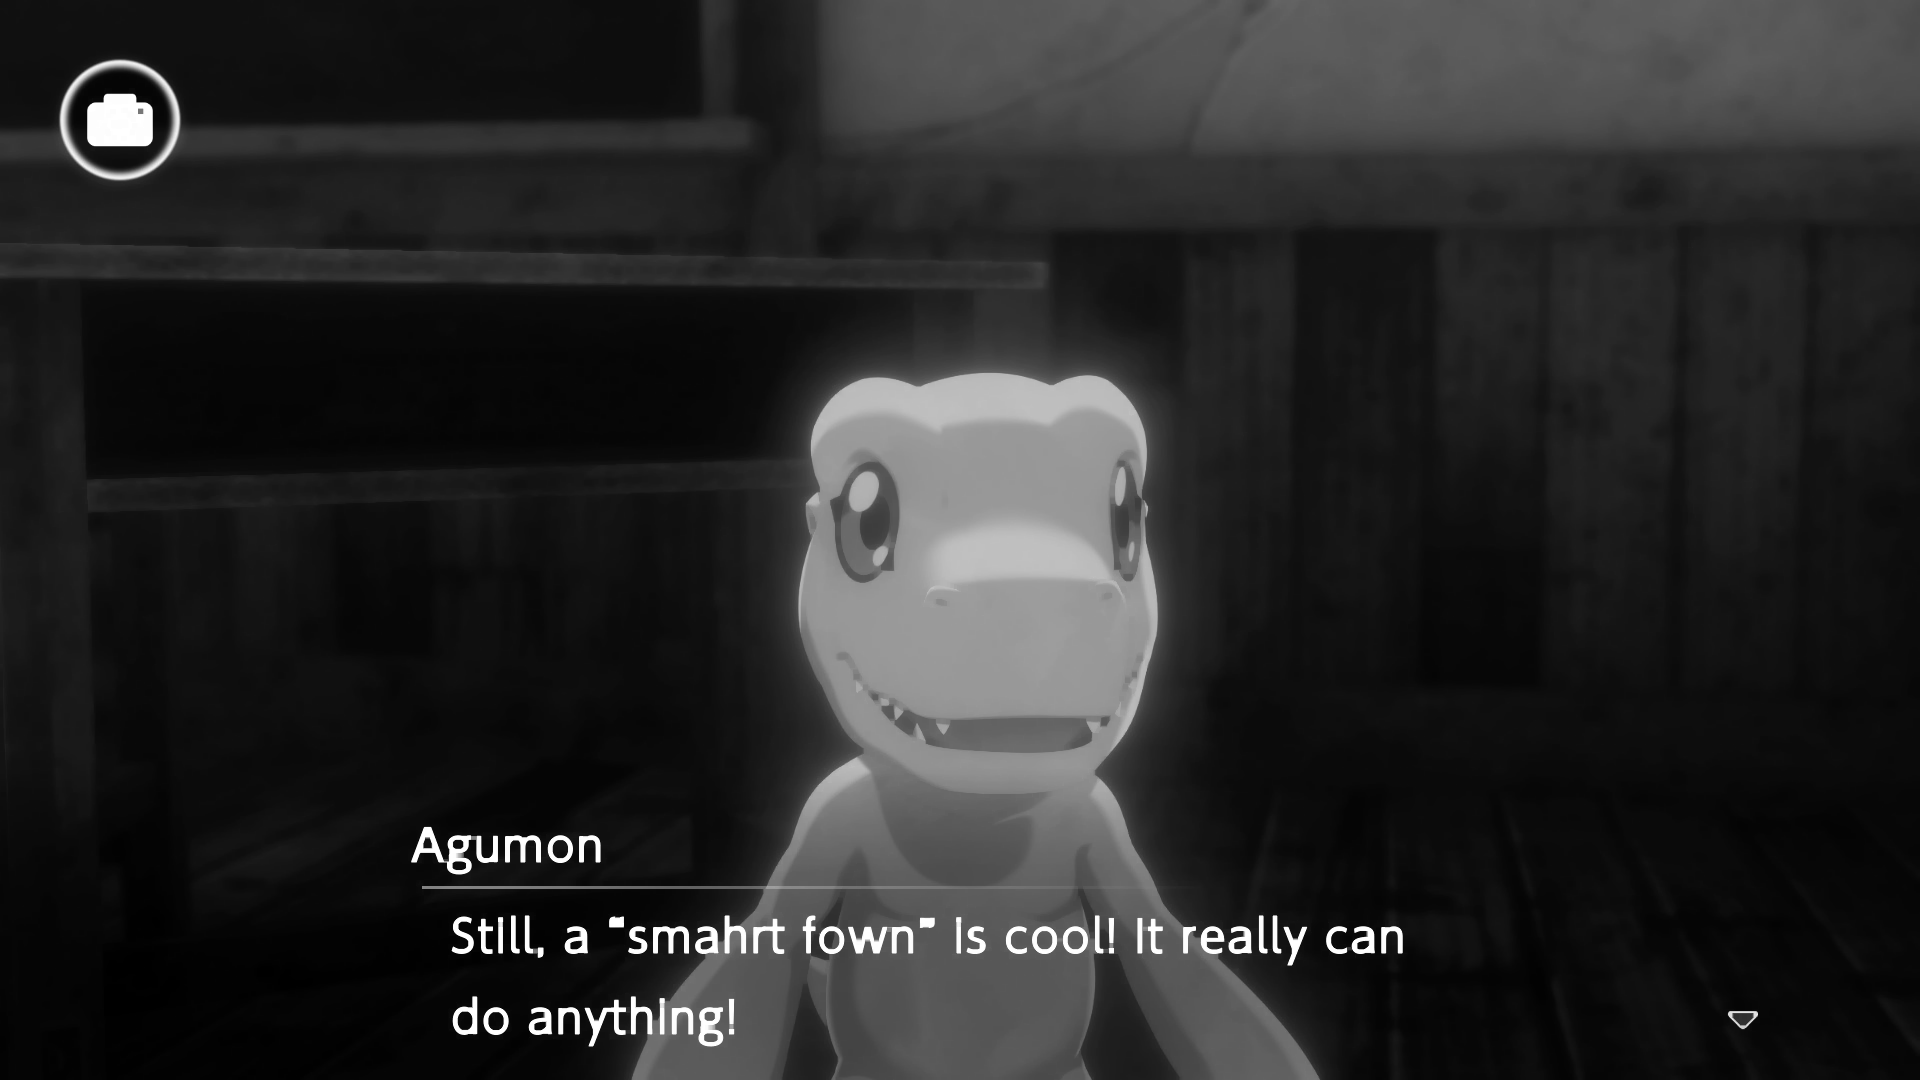
\includegraphics[width = 0.5\textwidth]{Imagenes/Preprocesado/10.png}
	\end{figure}
	
	\item \textbf{Denoising} (Reducción de ruido): 
	Elimina o reduce el ruido en una imagen para mejorar la calidad visual y el rendimiento de tareas de reconocimiento.
		\begin{figure}[H]
		\centering
		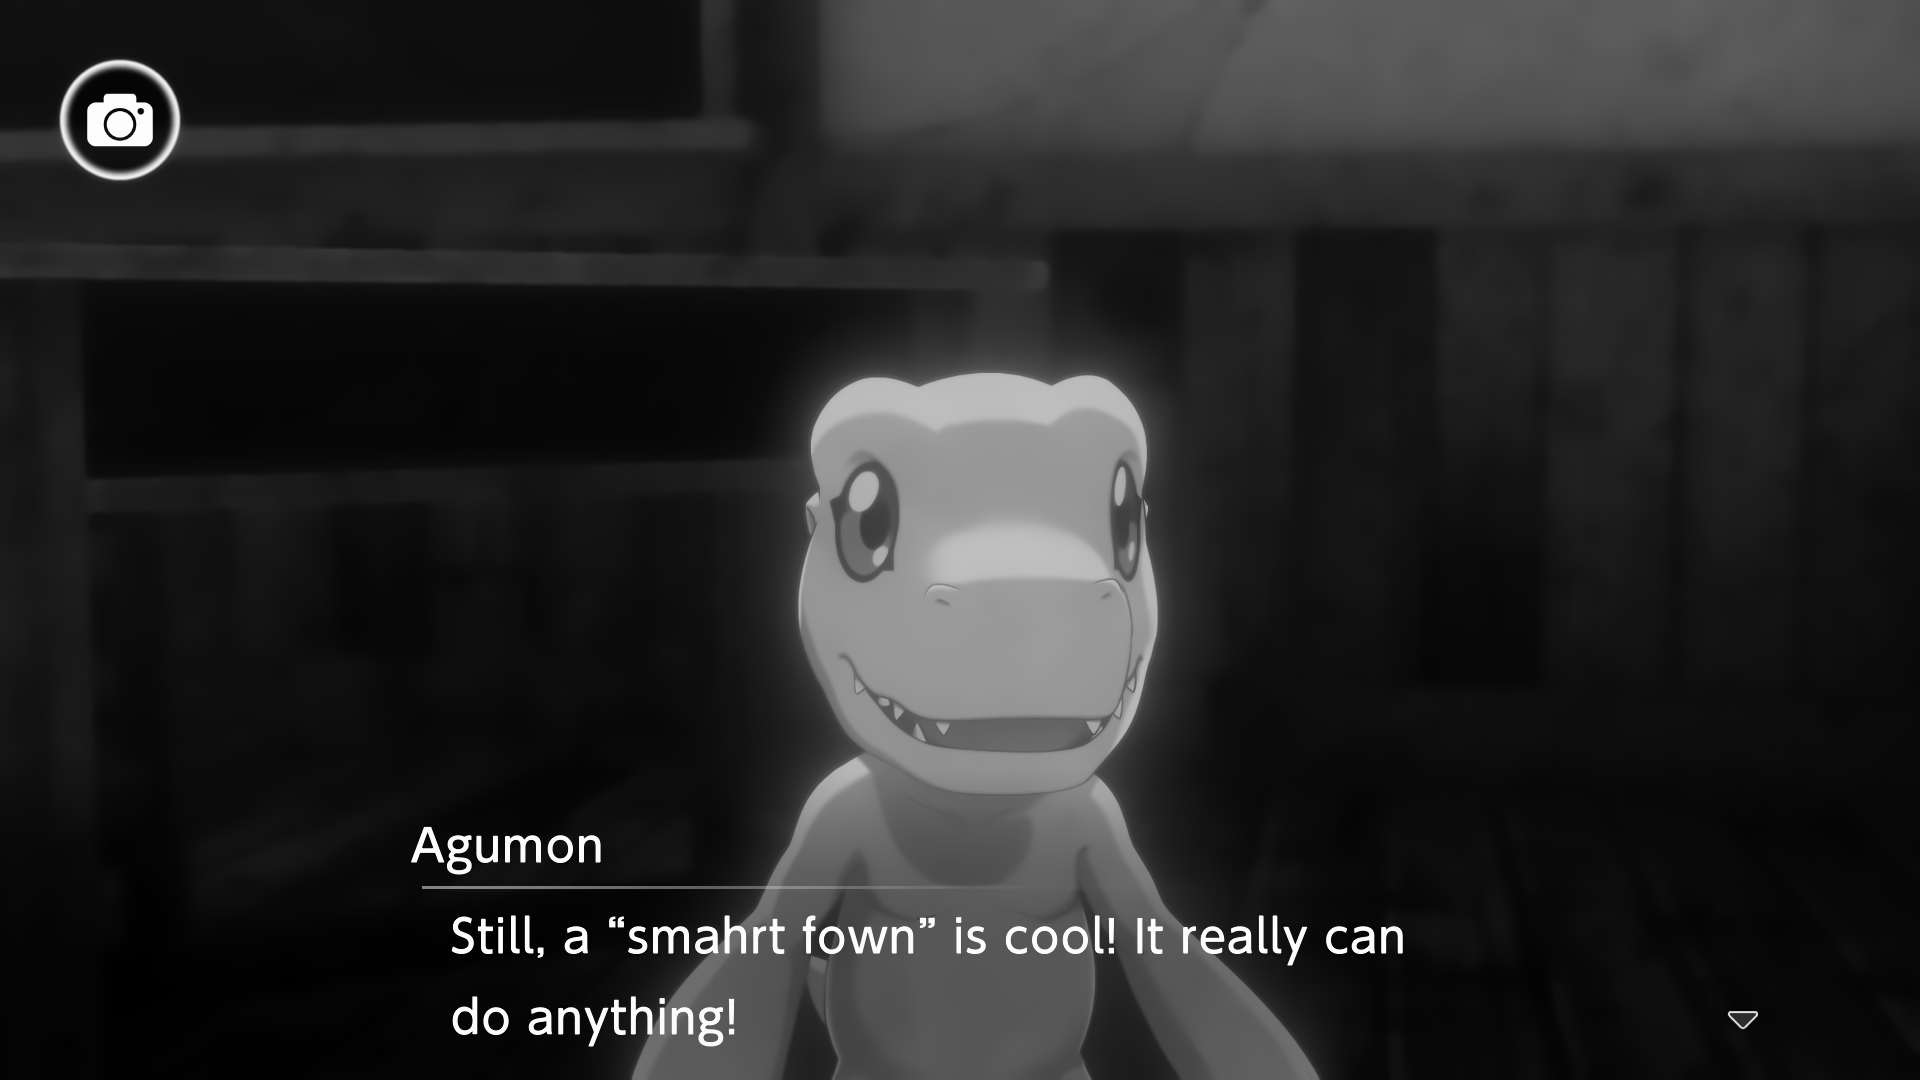
\includegraphics[width = 0.5\textwidth]{Imagenes/Preprocesado/11.png}
	\end{figure}
	
\end{enumerate}
Resultados obtenidos con los distintos tipos de preprocesamiento en cada categoría de imágenes.
\begin{table}[H]
	\begin{tabular}{llllll}
		Tipo                                                                 & Complejo                      & Simple                       & PixelArt                      & TxTBoc                       & TxtBoc2                       \\
		Grises                                                               & 3.72                          & 0.59                         & 2.69                          & 1.17                         & 2.16                          \\
		Contraste                                                            & 5.06                          & 0.81                         & 2.39                          & 1.13                         & 10.07                         \\
		\begin{tabular}[c]{@{}l@{}}Ecualización\\ de histograma\end{tabular} & 5.59                          & 3.60                         & 6.56                          & 2.41                         & 8.67                          \\
		Gamma                                                                & 3.72                          & 0.59                         & 2.69                          & 1.17                         & 2.16                          \\
		Filtro de nitidez                                                    & 11.06                         & 2.17                         & 8.84                          & 3.29                         & 12.05                         \\
		Thresholding C                                                       & \cellcolor[HTML]{FF0000}16.80 & \cellcolor[HTML]{FF0000}9.44 & 10.36                         & 4.08                         & \cellcolor[HTML]{FF0000}23.44 \\
		\begin{tabular}[c]{@{}l@{}}Thresholding\\ Gaussian\end{tabular}      & 12.85                         & 9.35                         & \cellcolor[HTML]{FF0000}16.16 & \cellcolor[HTML]{FF0000}4.71 & 22.83                         \\
		Thresold Binary                                                      & 4.05                          & \cellcolor[HTML]{00FF00}0.49 & 2.14                          & 1.79                         & 2.04                          \\
		\begin{tabular}[c]{@{}l@{}}Redimension\\ x1.5\end{tabular}           & 4.77                          & 0.80                         & 2.86                          & 1.27                         & 3.07                          \\
		Gaussian Blur                                                        & 3.02                          & 0.68                         & 2.34                          & 1.14                         & 1.86                          \\
		Median Blur                                                          & 2.75                          & 0.51                         & 2.75                          & 1.25                         & 1.37                          \\
		2 Blur                                                               & 2.26                          & 0.59                         & 2.15                          & 1.22                         & \cellcolor[HTML]{00FF00}1.09  \\
		Dilatación y erosión                                                 & 2.19                          & 0.51                         & 2.48                          & \cellcolor[HTML]{00FF00}0.69 & 1.83                          \\
		Dilatación                                                           & \cellcolor[HTML]{00FF00}1.80  & 0.62                         & \cellcolor[HTML]{00FF00}1.23  & 0.80                         & 5.53                          \\
		Erosión                                                              & 2.02                          & 1.00                         & 2.57                          & 0.82                         & 1.21                          \\
		Denoising                                                            & 3.23                          & 0.57                         & 2.64                          & 1.07                         & 1.70                         
	\end{tabular}
\end{table}

El CER en este caso supera al 1 debido a que el OCR reconoce más caracteres de lo que hay en el ground-truth, es decir, reconoce muchos caracteres "basura".

Se marca en rojo aquel tipo de preprocesamiento que da peor resultado en la categoría y en verde, aquel que da mejor resultado.

Obteniendo esta tabla y viendo los resultados de imágenes se ha ido probando distintas combinaciones de preprocesados de imágenes y se ha obtenido la siguiente combinación:
\begin{itemize}
	\item Grises
	\item Escalado
	\item Simple Threshold
	\item Denoising
	\item Blurring
	\item Dilate\_Erode	
\end{itemize}
Obteniendo estos resultados:
\begin{table}[H]
	\begin{tabular}{lllll}
		Complejo & Simple & PixelArt & TxTBoc & TxtBoc2                      \\
		2.57     & 0.29   & 2.01     & 1.01   & 1.49
	\end{tabular}
\end{table}
\subsection{Eliminación de caracteres basura}
Una posible salida de la OCR puede ser la siguiente:

\begin{verbatim}
	YRNY L., R Y .
	t ::;h.'. . ,’_:“?; -' [
	Y& i AT
	A DU T AR BIE
	e vl e \-' .: ’4 -7
	g ... . ‘s "
	_-'.‘_;g ""M“ a DO .
	* v o ‘ >
	e \1 v we » r
	—,:)‘“ - ~ ‘ S " v - .
	- ’ p S A ’ -t » e . -~
	) p '_" - Y . 4 ) ) e “ ",
	RS g~ C okl A e .
	o “\ ., ":.-.. _x '.- - — "- : ' . 1'1 N .»rv
	TN A foow. TREELYS 4 e
	v\ U - ' b.""*— .
	. . ) . ‘ . J - . h v ’k‘ Py
	Mo . : . ¢ . . . .
	. ’/. . A.; ‘-\ ' .
	it - g 03: b 4
	7 - ] > I »“ Y “. Pl
	L It's been a long road. You have the right to stretch your legs!
	L2 p
	’ - . r £ . R ¥ h N\
	y /’ - . J ’ ‘- - .i;" N
	
\end{verbatim}
Donde la frase que realmente importa es solamente una o dos líneas de la salida
\begin{verbatim}
		L It's been a long road. You have the right to stretch your legs!
\end{verbatim}
Esto es un problema importante que debemos solucionar ya que es imposible saber si un test es correcto o no con esta entrada.

En esta sección se propone una solución a este problema de caracteres ``basura'' usando el algoritmo\footnote{(Algoritmo para C++ Levenshtein distance)\url{https://github.com/guilhermeagostinelli/levenshtein/blob/master/levenshtein.cpp}} de distancia \emph{levenshtein}.

La distancia de Levenshtein\footnote{(Levenshtein distance Wikipedia) \url{https://en.wikipedia.org/wiki/Levenshtein_distance} } (también conocida como distancia de edición) es una métrica utilizada para medir el grado de diferencia entre dos cadenas de texto. Específicamente, se define como el número mínimo de operaciones necesarias para transformar una cadena en otra, utilizando tres tipos de operaciones básicas:
\begin{itemize}
	\item Inserciones: Agregar un carácter.
	\item Eliminaciones: Eliminar un carácter.
	\item Sustituciones: Reemplazar un carácter por otro.
\end{itemize}

Suponiendo que tenemos el texto esperado de la imagen,  utilizando esta métrica, podemos obtener la distancia levenshtein entre una línea del texto esperado y una línea del texto reconocido por la OCR. Con la distancia obtenida y aplicando un cierto umbral, podemos identificar aquellas líneas que más se asimila al texto esperado, obteniendo así las líneas deseadas y descartando aquellas que no cumpla un cierto umbral.

Uno de los resultados obtenidos aplicando la distancia levenshtein es la siguiente:
\begin{itemize}
	\item Texto esperado:
	
	\begin{verbatim}
		Agumon
		Still,a "smahrt fown" is cool! It really can
		do anything!
	\end{verbatim}
	\item Texto real de OCR:
	
		\begin{verbatim}
	"
	|
	\ J
	—
	Agumon /
	Still, a “smahrt fown” is cool! It really can
	do anything! <
	\end{verbatim}
	\item Texto aplicando distancia levenshtein:
	\begin{verbatim}
	Agumon Still smahrt fown is cooll It really can do anything
	\end{verbatim}
\end{itemize}  
Obteniendo estos nuevos resultados en el CER medio:

\begin{table}[H]
	\begin{tabular}{llllll}
		Tipo        & Complejo & Simple & PixelArt & TxTBoc & TxtBoc2                      \\
		OCR         & 2.57     & 0.29   & 2.01     & 1.01   & \cellcolor[HTML]{FFFFFF}1.49 \\
		Levenshtein & 0.63     & 0.16   & 0.63     & 0.55   & 0.42                        
	\end{tabular}
\end{table}
\section{Descripción de los tests}




\subsection{Evaluación sobre problema de fuente (Error \ref{ErrorFuente})}


\subsection{Testing sobre idioma incorrecto}


\subsection{Testing sobre solapamiento de texto (Error \ref{ErrorSolapamiento})}
Para resolver este problema se plantea usar el OCR para detectar las posiciones de los textos, seguido de una librería gráfica para detectar el contorno de la caja delimitadora guardado para ese texto, y obtener así sus posiciones. Comparando la posición del texto y la posición de la caja delimitadora obtenemos si el texto se está saliendo de la caja o no.
	
Para simplificar el test, damos algunas restricciones: 
\begin{itemize}
	\item En la imagen, el texto tiene que aparecer completamente en horizontal sin ninguna rotación sobre el eje X.
	\item Detectamos texto que sobresale por los lados.
	\item Al ser un botón, tiene que estar resaltado y tener un claro contraste con el fondo y el texto para facilitar la detección
	\item Debe tener una forma de caja o ventana(cuadriculada, cuadriculada redondeada), no sirve, por ejemplo, un bocadillo en forma de nube.
\end{itemize} 
	
\subsection{Testing sobre detección de placeholders}


\subsection{Testing sobre truncamiento de texto (Error \ref{ErrorTruncamiento})}


\subsection{Testing sobre error tipográfico (Error \ref{ErrorTypo})}


\subsection{Testing sobre error gramatical (Error \ref{ErrorGramatical})}

 

